\documentclass[11pt,twoside]{report}
\usepackage{setspace}
%\singlespacing
\setstretch{1.25}
%\onehalfspacing

%--------------------
% Load all pacakges in the UsePackages.sty file
\usepackage{UsePackages}

\usepackage{titlesec}
\titleformat{\chapter}[display]   
{\normalfont\huge\bfseries}{\chaptertitlename\ \thechapter}{20pt}{\Huge}   
\titlespacing*{\chapter}{0pt}{0pt}{40pt}

\begin{document}


%--------------------
% TITELPAGINA EN INLEIDENDE PAGINA'S

\begin{titlepage}
\vspace*{10mm}

          \begin{figure}[H]
                \centering
              
\includegraphics[width=0.9\linewidth]{TitlePage/TUe-logo-descriptor-line-scarlet-L.png}
          \end{figure}

\begin{center}


\vspace*{15mm}

    \Huge
    \textbf{Model-based control for soft robot manipulation\\}
    
\vspace*{10mm}   
    \Large
    {M.W. IJpelaar} \\
    {0958812}
    
    
\vspace*{2.5cm}
\large
 \textbf{Supervisors:}   \\
    ir. B.J. Caasenbrood   \\
    dr. A.Y. Progromsky  \\
    prof. dr. H. Nijmeijer   \\

\vspace*{25mm}

\end{center}

\begin{flushleft}
Eindhoven University of Technology \\
Department of Mechanical Engineering \\
Dynamics \& Control
 
 
\vspace*{5mm} 


Eindhoven, Netherlands\\
\today \\
DC 2021.XXX
\end{flushleft}
	
	
\end{titlepage}
\thispagestyle{empty}
%\cleardoublepage


\pagenumbering{roman}

\chapter*{Abstract}
In the past decades, the field of soft robotics has been receiving a substantial amount of research interest. In contrast to their rigid counterparts, soft robots distinguish themselves as intrinsically dexterous, flexible and resilient. These inherent properties can reshape our perspective on robotics. Their potential is readily acknowledged in the fields of medical sciences and co-robotics. 



In this work, soft robots applied for object manipulation are considered. Recent advancements have led to a novel technique of modelling soft robots by exploiting partial differential equations. This method allows to accurately describe, the possible complex, configurations employing a continuous curve. The theoretical infinite degree-of-freedom soft robotic system is reduced to a finite-dimensional model equivalent by exploiting the Galerkin reduction method. This allows the application of well-established theories, including Lie group theory, to derive a dynamic model. In this study, the proven method of Jacobian transposed control is transferred to the domain of soft robotics. The performance of this feedback controller is evaluated for simulated dynamic responses and experiments conducted on a physical setup. The achieved results demonstrate that Jacobian control can be considered a valuable alternative over more advanced model-based control methods.
\cleardoublepage

\tableofcontents

\cleardoublepage
\textbf{\large Nomenclature}

\begin{multicols}{2}



























\end{multicols}
\cleardoublepage


%--------------------
% HOOFDTEKST 


\pagenumbering{arabic}



\chapter{Introduction}
\label{chapter1}

In recent years, the field of soft robotics has received a substantial increase of research interest \cite{iida2011soft},\cite{walker2020soft}, \cite{bao2018soft}. Soft robots cover a vast domain for suitable application. This includes the medical field \cite{sitti2018miniature} \cite{ashuri2020biomedical}, where soft robots have potential applications in artificial muscles, prosthetic devices, stents and surgical instruments. They can also be applied to explore places that are almost impossible to reach for human beings. This includes offshore operation and deep-sea exploration \cite{aracri2021soft}, such as the soft robot exploring the depths of the Mariana trench \cite{laschi2021soft}. Other applications are in the field of industrial automation, where they can support human operators in manipulating objects \cite{george2018control}, \cite{grissom2006design}. A variety of experimental soft robots are displayed in Figure \ref{fig1:softexample}. 



\begin{figure}[H]       
    \centering
    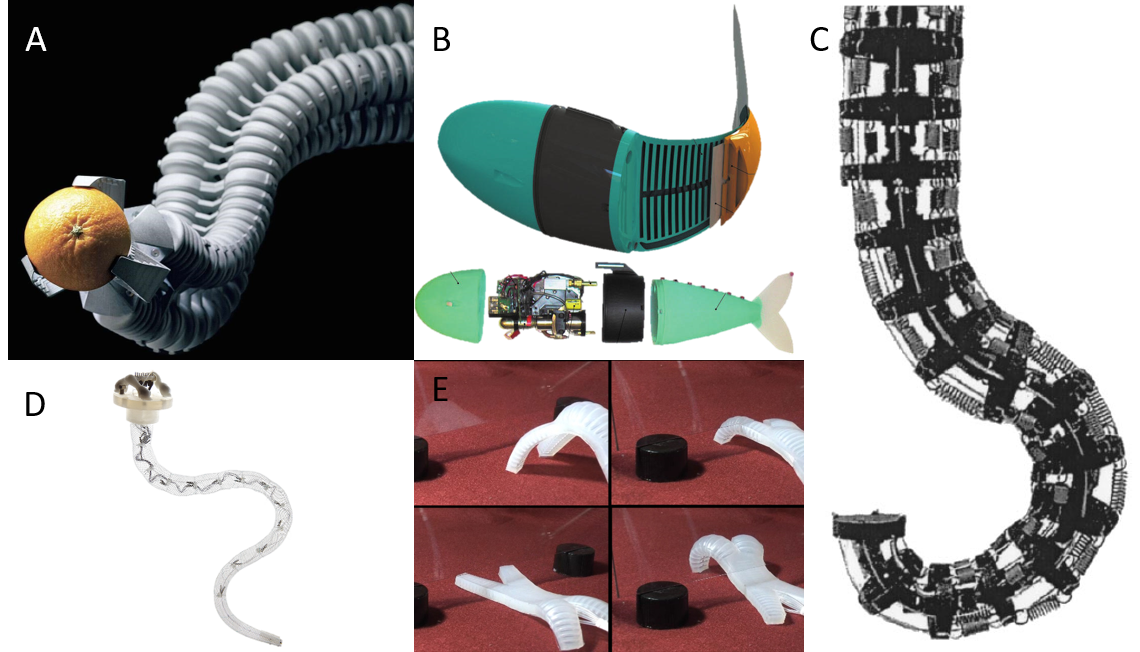
\includegraphics[width = \textwidth]{Figures/Chapter1/robotexamples.png}
    \caption{\textbf{A}: Bionic Handling Assistant inspired by the trunk of an elephant \cite{BHA}. \textbf{B}: Bio-inspired soft robot replicating movement of a fish \cite{marchese2014}. \textbf{C}: Elephant’s Trunk Manipulator \cite{hannan2003kinematics}. \textbf{D}: Bio-inspired soft octopus tentacle \cite{laschi2012soft}. \textbf{E}: Pneumatically actuated starfish-like soft robot \cite{shepherd2011multigait}.}
    \label{fig1:softexample}
\end{figure}


The foundation of soft robotic design is often found in nature and includes inspiration for material choice, locomotion, and morphology. As their name already suggests, soft robots are made from soft and flexible materials. Their inherently dexterous structure allows soft robots to easily manoeuvre around obstacles. This makes soft robots robust and very applicable in constantly changing environments. A few examples of bio-inspired soft robots include emulated trunks \cite{hannan2003kinematics} inspired by the proboscis of an elephant, robots based on the arm of octopus \cite{wang2013visual}, and robots that replicate the movement of fish \cite{marchese2014}, Figure \ref{fig1:softexample}. 


\subsection*{Soft robot manipulators vs. traditional manipulators }

This thesis restricts itself to soft robots designed for manipulating objects. These robots reshape the idea of using robots for industrial processes. Currently, rigid robots dominate the field of industrial automation, as they excel in accuracy, repeatability and load capacity. However, these traditional robots tend to be unsafe when operating in human-centred environments. Classic robots are composed of rigid materials and accelerate to high velocities, which could create an unsafe environment for human operators. Additionally, these robots have limited degrees of freedom, making it harder to avoid obstacles. To evade the risk of potential harm, and create more dexterous robots, innovative soft robotic manipulators are designed. Since these robots are composed of soft materials they are inherently safer to operate around humans. However, due to their flexible nature, they show different dynamic behaviour compared to traditional robots. To gain a better understanding of soft robotic manipulators, parallels are drawn and differences are mentioned between soft robot manipulators and traditional robots: i) material, ii) actuation, iii) sensing.


First, a classification is made based on the compliance of their underlying materials \cite{Bionics2008}. Generally, classic robots are made of rigid metal beams, whereas soft robots are made from soft polymer materials. The building materials of the robot largely determine the kinematic redundancy of the robot. Since soft robots are composed of materials with an extremely low Young's modulus, they can sustain large (and possibly non-linear) deformation during normal operation. As a result of this compliance, gravity and payload cause a distributed deformation throughout the entire system. Therefore, these soft robots have a theoretical infinite amount of degrees of freedom. This makes soft robotic control more challenging when compared to traditional robots, as the latter has a fixed amount of degrees of freedom.

Secondly, actuation is a major difference between the two robot types. Whereas traditional robots are generally electro-mechanically actuated, soft robots can be actuated with a wide range of actuation methods, which includes pneumatics, hydraulics, thermal and even chemical \cite{BHA},\cite{marchese2014},\cite{kang2019programmable},\cite{shepherd2013using}. Rigid robots are often linked by rotatory or prismatic joints, where its design allows to include the actuator inside the robot's casting or joint. The actuators of soft robots are often located externally, as their design simply does not allow to integrate them. Most soft robot manipulators are actuated pneumatically or by using variable-length tendons \cite{Rus2015}. A well-known example of a pneumatically actuated soft robot is the Bionic Handling Assistant (BHA) by Festo, as shown in Figure (\ref{fig1:softexample}). This type of soft robot has inflatable channels that cause deformation when applying pressure. An example of a tendon driven robot is the elephant trunk's robot \cite{cieslak1999elephant} (Figure \ref{fig1:softexample}). This manipulator consists of eight elastic segments linked together by coil springs. Each segment is controlled by two pairs of strings. Servo or linear actuators are used to wind and unwind the strings, with that controlling the movement of the robot. Both actuation methods introduce additional dynamics largely affecting the performance of the entire control system. 

Thirdly, conventional sensing mechanisms can often not be applied to soft robots. For hard robots, the joint design often allows incorporating encoders to measure rotation and other sensory devices. Since the forward kinematics, given rigid joints and links, can be computed through trigonometry, position sensing is relatively easy. For soft robots, the compliant and lightweight nature often prevents the integration of conventional sensors, such as encoders, strain gauges and inertial measurement units (IMU's) \cite{Rus2015}, \cite{Lee2017}. Alternative sensory techniques are often needed. These methods include for instance optical sensors and stretch sensors based on macrobend fibres \cite{Sareh2015}.

\subsection*{Control strategies}

The aforementioned discussed the contrast between rigid robots and soft robots. It showed that soft robot manipulators distinct themselves from traditional robots on three fronts. Their inherent soft body leads to a theoretical infinite degree system. The actuation of soft robots introduces additional dynamics caused by the actuators. Furthermore, the conventional sensory mechanisms can often not be applied to soft robots, and therefore demand more complex sensory devices. These factors combined, majorly affect the control of soft robots. Recent literature often tries to convey readily available control theories adopted on traditional robots and apply those to soft robotics.

The work of Thuruthel et al. (2018) \cite{george2018control} presents an overview of recent findings in soft robotic control for pneumatically actuated and tendon-driven soft robots. In the mentioned work, three control approaches are distinguished, namely model-free, hybrid and model-based control. A model-free control strategy does not use a kinematic or dynamic description in its control approach. Instead, it exploits learning-based algorithms to dynamically control the robotic system. Hybrid controllers combine learning or empirical elements with a model-based approach. The model-based controllers rely on an analytical description of the robotic system. Furthermore, for each control approach, a sub-division between kinematic and dynamic control is made. Kinematic control is defined as a zero-order input-output relation. This implies that a change in input is directly observed in output. Therefore, this approach is lower-level compared to dynamic control. For the latter, the configuration space and/or task space variables' velocities are used in the control algorithm. 


Research conducted on the Bionic Handling Assistant, as shown in Figure \ref{fig1:softexample}, demonstrates that multiple control methods can be applied to the same robot. A model-free control approach was implemented in \cite{rolf2013efficient}. The inverse kinematics of the robot were obtained through machine learning, instead of model-derivation. Later work shows the implementation of a hybrid controller \cite{reinhart2017hybrid}. In this approach, an inverse kinematic model was used together with a learning model. Previous to this hybrid controller, a model-based controller was proposed by \cite{mahl2014bhakin}. However, this model-based controller only used a kinematic description of the soft robot. This research was followed up by \cite{falkenhahn2016dynamic}, which developed a dynamic controller. In this latter work, the system is controlled with a nonlinear length controller based on feedback linearization. This controller was further supported by linear PD and feedforward control. 

In \cite{wang2013visual} visual servo control is used to control a cable-driven soft robotic manipulator. The manipulator, inspired by an octopus' tentacle, is shaped like a cone. On the outer surface of the soft robot four cables are uniformly distributed. Each end of these cables is connected to the tip of the manipulator. The other end of the cables is connected to pulleys. By winding and unwinding the cables on the pulleys, the end-effector can be positioned in the task-space. A kinematic-based servo controller is designed, based on linear PD feedback control with gravity compensation. Position sensing is done by a camera mounted at the tip of the robot, and a fixed feature point. Based on this visual information, a Jacobian matrix is estimated, which is used in the kinematic controller.

In \cite{zhang2017visual} also visual servo control was implemented to control a tendon-driven soft robotic manipulator. Again, kinematic control is used for a reference tracking problem. In the mentioned work, the Jacobian is calculated by a FEM model operating in parallel. The reference input is feed through the FEM model, outputting a Jacobian matrix and expected end-effector position. The Jacobian is used in the controller to control the actual manipulator. The FEM model's expected end-effector position and actual end-effector position are used in a second controller to enhance Jacobian estimation in the FEM model.

A model-based controller that uses a dynamic model in its control loop is presented in \cite{della2020model}. The robots infinite dimensionality is resolved by regarding the robot being composed of six individual actuatable segments. A piece-wise constant curvature (PCC) approach was used to describe the kinematics of the robotic actuator. For each segment, Denavit-Hartenberg (DH) parameters are used to describe the rigid robot equivalent, which is then used to derive a dynamic model. Essentially, the proposed controller is a computed-torque controller with an additional PD controller. 

\subsection*{Modeling of soft robots}

In the aforementioned work, \cite{della2020model}, the infinite dimensionality of the soft robot is solved by assuming the robot consists of a fixed amount of segments. In this way, the infinite degree-of-freedom system can be approximated by a fixed amount of degrees of freedom. This makes controller design easier. Of course, the reduction of degrees of freedom is at the cost of model accuracy. In the work of \cite{della2020model}, the PCC modelling approach was applied. This is a widely adopted method for describing the configuration of soft robots \cite{ccapproach}. This modelling approach can be applied to soft robots that undergo a very specific deformation. Previous research that used this model include \cite{mahl2014bhakin},\cite{ccapproach},\cite{berkers},\cite{Falkenhahn2015},\cite{runge2017framework}. A schematic drawing of the constant curvature modelling approach is shown in Figure \ref{fig2:ccapproach}. Although our modelling approach distinguishes itself from this methodology, it is important to grasp the basics. 

The constant curvature describes the position of the actuator by three coordinates. Parameter $l$ is the curved length of the actuator measured from the fixed bottom to the tip. Coordinate $\kappa$ expresses the curvature of the actuator. It is assumed that the deformed actuator describes a perfect arc, hence radius $r$ is equal to $\frac{l}{\kappa}$. This allows writing the orientation of the actuator's tip as $\theta = l\kappa$. Lastly, parameter $\phi$ describes the rotation of the actuator relative to the ground. A single constant curvature is not able to describe complex actuator configurations. To this end, multiple of these curves are stacked onto each other, thereby discretizing the actuator. This allows describing more complex configurations. This methodology is used in for instance \cite{Falkenhahn2015}.



\begin{figure}[H]
    \centering
    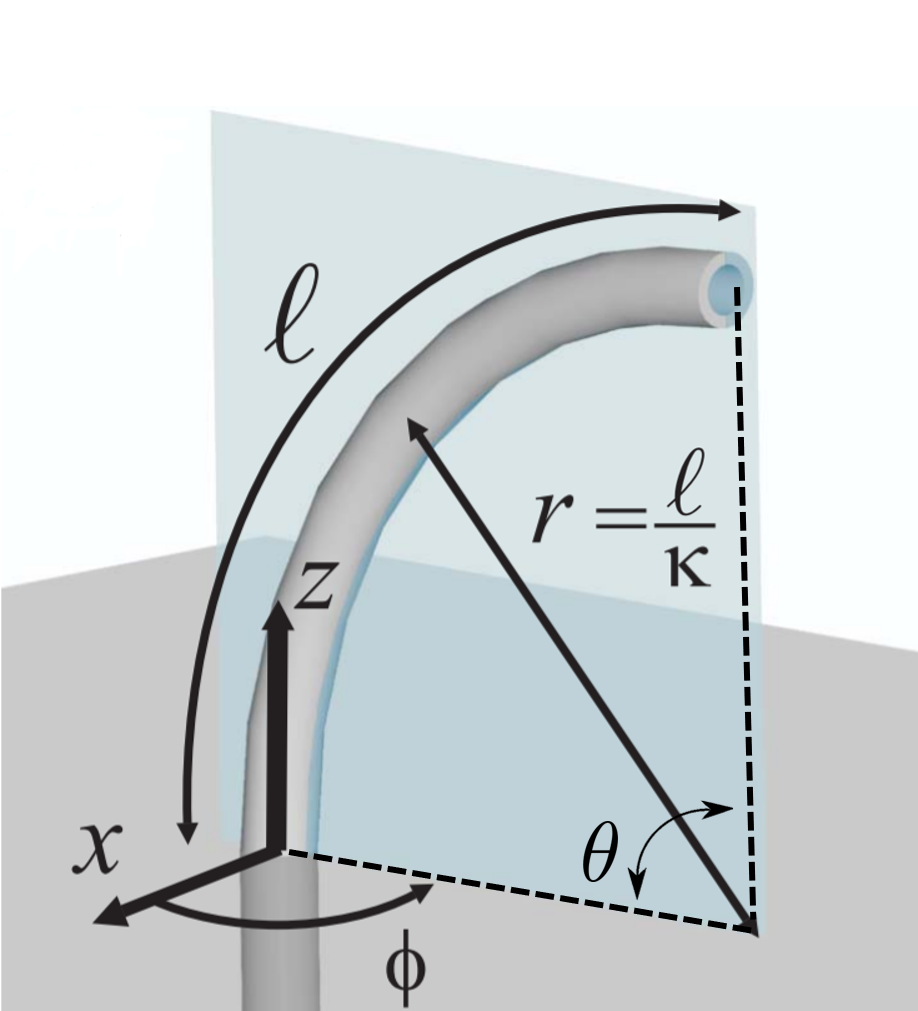
\includegraphics[width = 0.45\textwidth]{Figures/Chapter1/ccapproach2.png}
    \caption{Schematic drawing of the constant curvature model, adapted from \cite{ccapproach}.}
    \label{fig2:ccapproach}
\end{figure}

The PCC approach has some limitations, due to its piece-wise character the actuator configuration is not described by a single continuous function. This makes it harder to find analytical expressions e.g. derivatives. Additionally, this PCC approach only allows assigning material properties to particular points. This makes dynamic models generally less accurate. A method to overcome this problem is using partial differential equations (PDE's) to describe actuator configurations. These PDE's are more suitable for deriving continuum dynamic models. One of these models is the Cosserat beam model which will be exploited in this work. This Cosserat model describes the soft robot's configuration by a continuous curve. This continuous curve reflects strains in the backbone of the (deformed) soft robot. Approximation of these strains allows describing the system in a reduced-order form. The reduction of dimension enables dynamic model derivation for the soft robot. This dynamic model can then be utilized for model-based control purposes.


\begin{figure}[H]
\begin{minipage}{.5\textwidth}
  \centering
  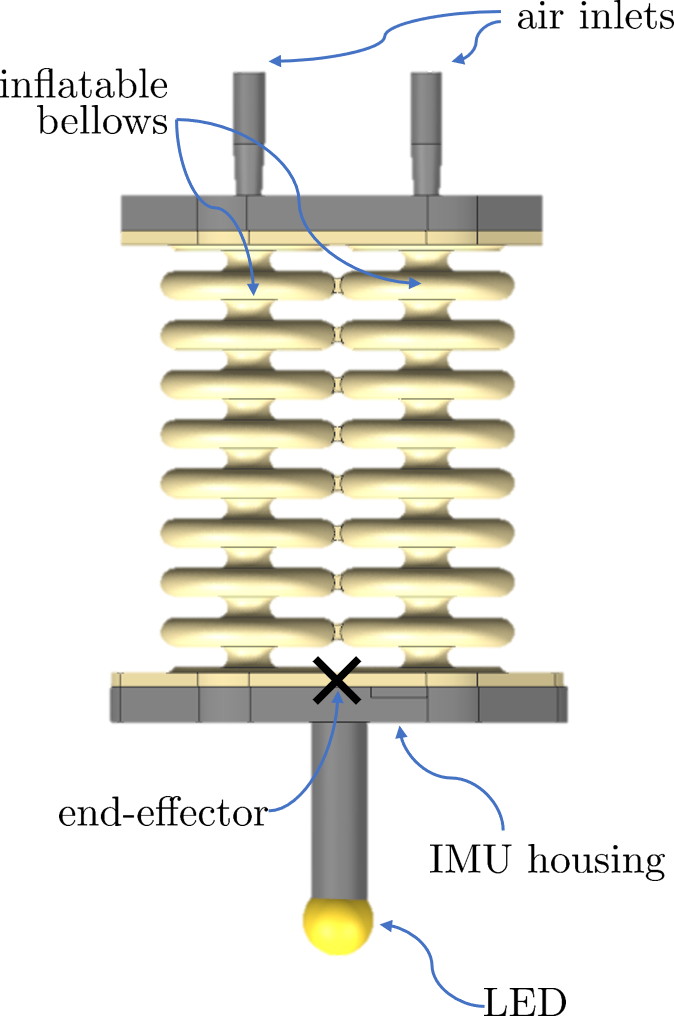
\includegraphics[width = 0.6\linewidth]{Figures/Chapter1/completesetup2.png}
  \caption{Computer rendered image of the soft robot setup }
  \label{fig:test1}
\end{minipage}
\hspace{10pt}
\begin{minipage}{.5\textwidth}
  \centering
  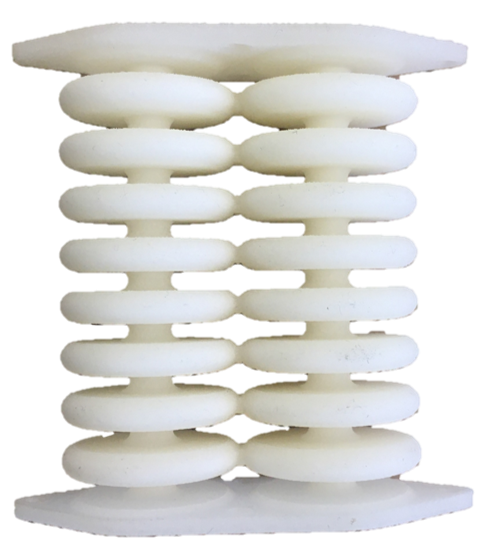
\includegraphics[width =0.6\linewidth]{Figures/Chapter1/actuator.png}
  \vspace{60pt}
  \caption{Planar soft robot, that can change its posture by inflating or deflating the bellows.}
  \label{fig:test2}
\end{minipage}
\end{figure}



\section*{Thesis outline and contribution}

In this work, we study the modelling and control of a planar soft robot as shown in Figure \ref{fig:test2}. This soft robot has a theoretically infinite amount of degrees of freedom, as it is composed of flexible polymer. Furthermore, it is pneumatically actuated, inducing additional dynamics into the control system, and is a major limiting factor on achievable control bandwidth. The soft robot consists of two individually inflatable bellows, allowing the robot to extend and curve. Each of the bellows can be inflated using air pumps. The induced rotation can be measured with an inertial measurement unit (IMU), which is mounted at the tip of the actuator. Using optical tracking, an LED marker connected to the tip of the robot can measure the elongation of the robot. The air pumps and sensory devices allow us to design a closed-loop controller, to perform set-point regulation. A schematic layout of the actuator setup is depicted in Figure \ref{fig:test1}.

This work is a continuation of the research of \cite{berkers}, which detailed a length and curvature controller for the planar soft robot. The mentioned work uses standard PD and PID control methods to ultimately perform a reference tracking problem. The obtained results are moderate for length and orientation control. However, the tracking performance is poor. To enhance the tracking performance of the system a model-based controller is proposed. The fundamentals of this research are provided in \cite{Caasenbrood2020}, which details a framework for modelling soft robot dynamics. This model is valuable for soft robotic control. Given the system description and previous research conducted on the planar soft robot, the research question that we try to answer is:

\textit{Can we develop a model-based control strategy for a pneumatically actuated, planar soft robot to perform a reference tracking problem?}



To effectively answer the research question several topics need to be considered. These topics are shown in the control layout of Figure \ref{fig1:controlarchitecture}. This control setup also shows the structure of this thesis. In Chapter \ref{chap2}, a forward kinematic description of the actuator is derived. This allows studying the robot's configuration in 2D space. Furthermore, it allows us to study the velocity of the actuator as a function of kinematic configuration. The latter allows us to derive a dynamic model of the actuator. Also, an air pump model is presented, which allows describing the entire system dynamics. Once this model is derived, a parameter study is performed in Chapter \ref{chap3}. Here, finite element analysis (FEA) is used to capture the non-linear stiffness of the soft robot. Furthermore, experiments are presented which allow determining the pump dynamics. In Chapter \ref{chap4}, a model-based controller is proposed. This controller will be tested in simulation, using the dynamic model as derived in Chapter \ref{chap2}. These simulation results, together with experimental verification are presented in Chapter \ref{chap5}.




\begin{figure}[H]
    \centering
    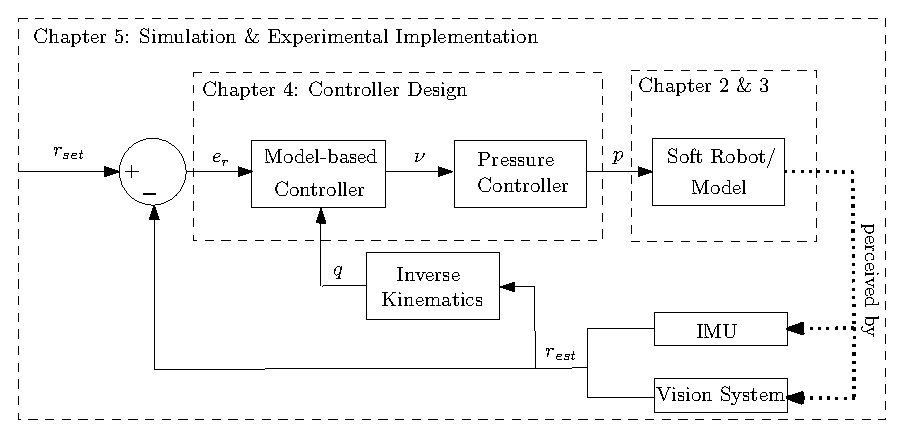
\includegraphics[width = \textwidth]{Figures/Chapter1/controlschemeCompleteGood.eps}
    \caption{Thesis layout and control setup.}
    \label{fig1:controlarchitecture}
\end{figure}


Recapitulating, this thesis comprises the following:


\begin{itemize}
    \item Chapter 2: Development of a non-linear dynamic soft robot model
    \item Chapter 3: Modeling of non-linear soft robot stiffness through finite element analysis
    \item Chapter 3: Experimental determination of air pump dynamics
    \item Chapter 4: Development of a model-based control law
    \item Chapter 5: Experimental implementation and simulation of a model-based controller
\end{itemize}



\cleardoublepage

\chapter{Dynamic Modeling}
\label{chap2}

This chapter describes the derivation of a dynamic model of the soft robotic manipulator. First, the soft robotic system used in this work is detailed. Then the configuration space of the soft robot is described. Once this configuration space is determined, the forward kinematics at position and velocity level are derived. These forward kinematics are useful for deriving the dynamic model of the soft robot. Additionally, a model is provided that is utilized to describe the pump dynamics. Lastly, the state-space representation of the overall system dynamics is presented, which combines the dynamics of the soft robot and pump dynamics.


%%%%%%%%%%%%%%%%%%%%%%%%%%%%
%%%%%%%%%%%%%%%%%%%%%%%%%%%%f

\section{System description}

The soft robot studied in this work is composed of a visco-elastic polymer using selective laser sintering technology. This manufacturing method is well suited to print hollow compartments, that allow for inflation. The elastomer has a low Young's modulus and can sustain large strains. These characteristics allow inducing large deformations with relatively low pressures. The geometry of the soft robot is best described by two bellows placed in parallel. Over the vertical axis, the bellows are connected, creating the centre line of the actuator. The bellows are connected by flanges at the top and bottom. The bellows can be inflated individually via air inlets created in the flange at one end of the actuator. The other end is closed, allowing to pressurize the bellows. Since each bellow can be inflated independently, the entire actuator can increase its length and change orientation. Pressurizing both bellows equally will result in a near pure elongation of the soft robot. Creating a pressure difference will cause the soft robot's upper flange to rotate. The following assumption is made concerning the robot's task space:

\begin{theorem}
Strains in the soft robot imposed by pneumatic actuation change the soft robot's length and orientation. Strains causing out of plane motion are deemed negligibly small, and can not be actively controlled. The soft robot's task space restricts itself to a single plane, reducing it to a 2-dimensional problem.


\end{theorem}

This assumption allows describing the configuration of the soft robot in a two-dimensional Cartesian plane. Since the soft robot has no clear end-effector in the form of a gripper, a point on the body is assigned to be the end-effector. This point is situated at the geometric midst of the closed flange, see Figure \ref{fig2:setup}. The flange with the air inlets is fixed, here its geometric midst is defined as the origin. Altering the bellow pressure can therefore change the soft robot's end-effector position. Based on the above assumptions a kinematic model of the soft actuator is developed using the Cosserat beam model. 



\begin{figure}[H]
\begin{minipage}{.5\textwidth}
  \centering
  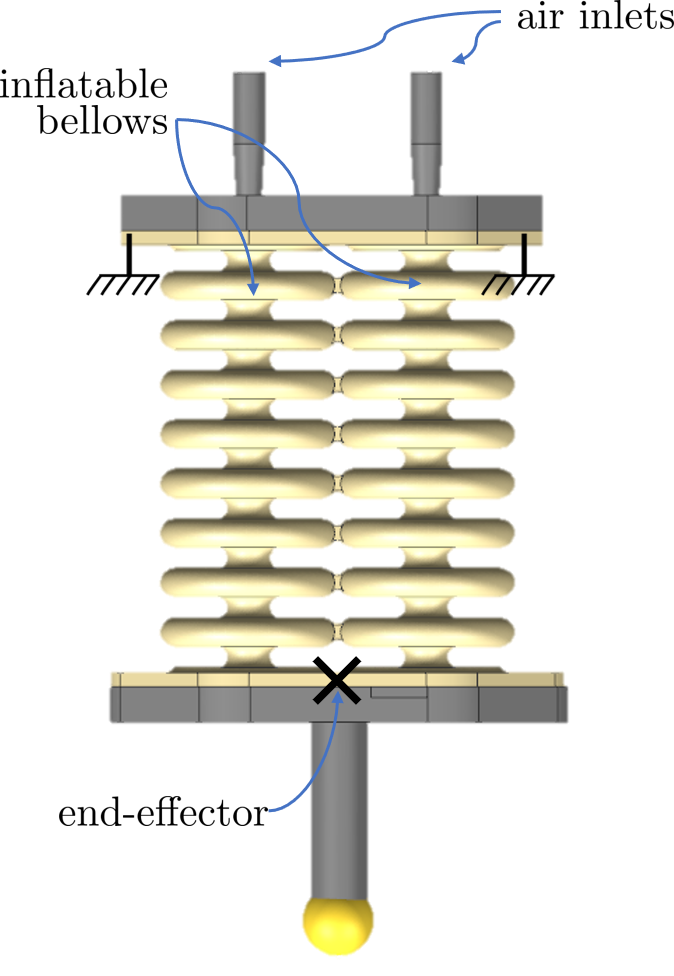
\includegraphics[width =0.8\linewidth]{Figures/Chapter2/setup.png}
  \caption{Schematic drawing of the actuator setup, denoting its fixation points and end-effector location.}
  \label{fig2:setup}
\end{minipage}
\begin{minipage}{.5\textwidth}
  \centering
    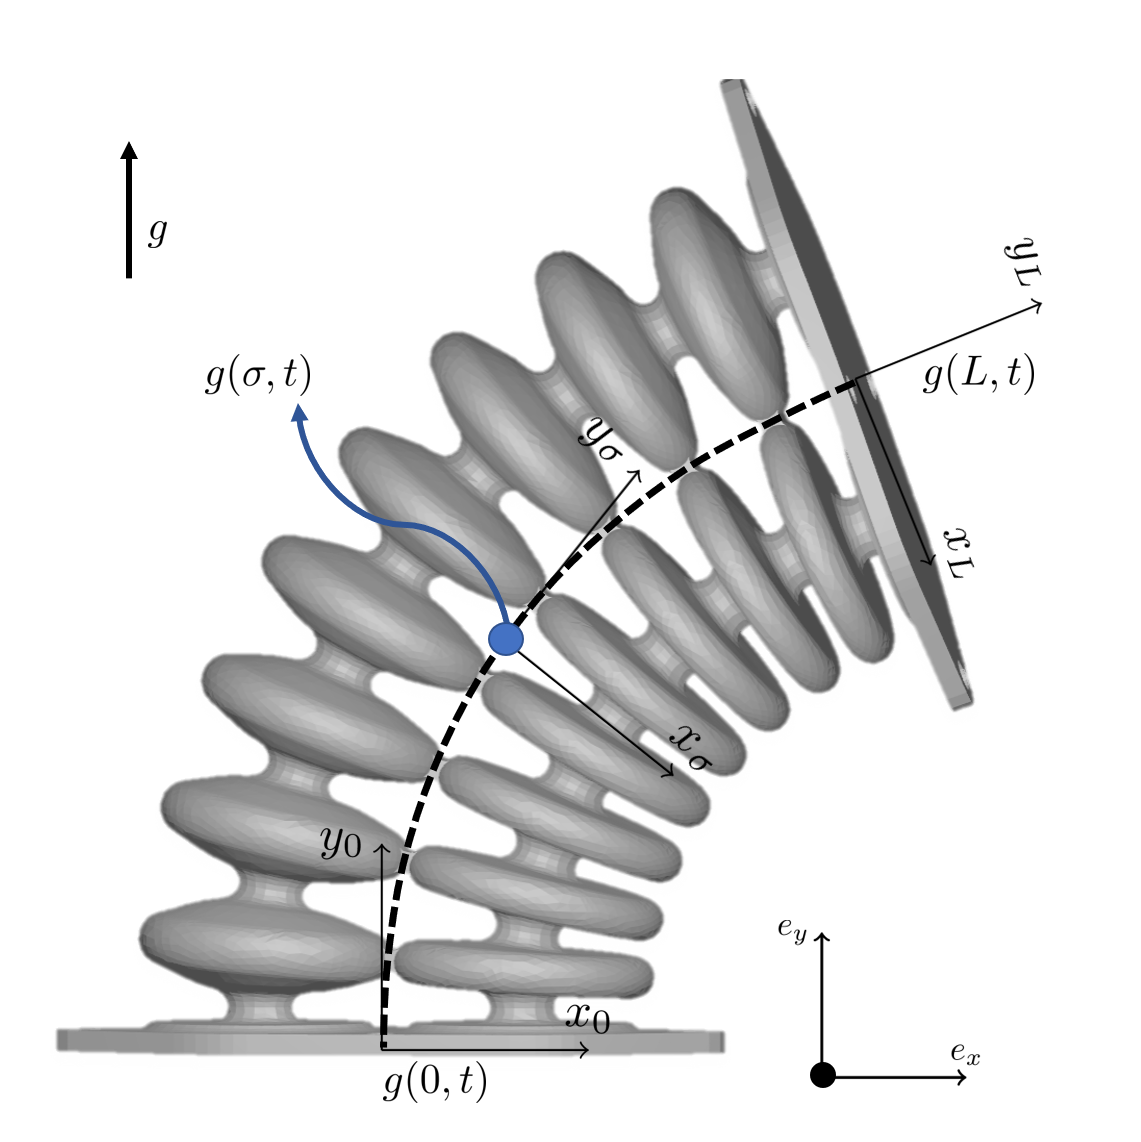
\includegraphics[width=\textwidth]{Figures/Chapter2/actuatorschematic.png}
    \vspace{15pt}
    \caption{Planar soft actuator with a two-dimensional backbone curve $g(\sigma,t)$.}
    \label{fig2:kinematicschematic}
\end{minipage}
\end{figure}





\section{Cosserat beam theory}

To describe the kinematics of the soft actuator, a Cosserat beam model is used \cite{Boyer2019}. This beam model can be thought of as a continuous one-dimensional curve representing the robot's backbone. This backbone is represented in Figure \ref{fig2:kinematicschematic} as the black dashed curve. This curve describes the configuration of the soft robot as a function of space and time. Therefore, this function is dependent on spatial coordinate $\sigma \in \mathbb{X}$ within bounded spatial domain $\mathbb{X} \in [0,L] \subset \mathbb{R}$, where $L$ is the relaxed manipulator length. Furthermore, a temporal coordinate $t \in \mathbb{T}$ with $\mathbb{T} \subset [0,T]$ is defined, where $T$ is the finite time horizon within the time domain. Under the assumption that the soft robot's task space is a two-dimensional plane, the rotation of any point $\sigma$ at time instance $t$ is given by rotation matrix $R(\sigma,t) \in \mathbb{SO}(2)$. The matrices in $\mathbb{SO}(2)$ represent the special orthogonal group within Lie group theory. This matrix allows to express rotation of points on a two-dimensional surface relative to the origin. Similarly, the position of that point is given by position vector $s(\sigma,t) \in \mathbb{R}^2$. Therefore, the Cosserat beam model creates a local frame at $\sigma$ tangential to curve $g(\sigma,t)$. This allows to describe position and rotation for any point $\sigma$ and time instance $t$ along the backbone of the soft manipulator by,


\begin{equation}
    g(\sigma,t) := \begin{bmatrix}  R(\sigma,t) & s(\sigma,t) \\ 0_2^\top & 1 \end{bmatrix} \in \mathbb{SE}(2),
    \label{eq2:g}
\end{equation}

where $\mathbb{SE}(2)$ represents the group of special euclidean matrices that represent rigid-body transformations on $\mathbb{R}^2$, namely rotations and translations \cite{Sola2018}. To derive forward kinematics, another assumption has to be made for this backbone curve $g(\sigma,t)$.

\begin{theorem}
Curve  $g(\sigma,t)$ is a continuously differentiable function on $\mathbb{T}$ and on $\mathbb{X}$
\end{theorem}

This assumption demands that derivatives of the backbone with respect to time and space are also continuous. These derivatives are essential in determining the strain and velocity field of the soft robot actuator. This strain field allows determining the time-invariant forward kinematics. Whilst the velocity field will be used in determining the system dynamics. First, we try to solve the forward kinematic problem by computing the strain field.



\section{Computation of the strain field}

The strain field allows us to study strains along the backbone curve. To find the strain we differentiate the backbone curve with respect to the spatial domain. Throughout this work derivatives with respect to the spatial domain will be indicated with a `prime', likewise time derivatives will be indicated with a `dot'. The local strain can be found by differentiating (\ref{eq2:g}) with respect to space. This results in the following partial differential equation (PDE), 

\begin{equation}
   g' = \frac{\partial g}{\partial \sigma} = g \hat{\xi} \hspace{10pt} \implies \hspace{10pt}  \hat{\xi}(\sigma,t) := g^{-1}g' = \begin{bmatrix} 0 & -\kappa & \epsilon_x  \\ \kappa & 0 & \epsilon_y \\ 0 & 0 & 0 \end{bmatrix} \in  \mathfrak{se}(2),
    \label{eq2:dgdsigma}
\end{equation}

where $\hat{\xi}(\sigma,t)$ is the space-twist field. Since the problem is planar, there is a single rotation. This rotation is described by curvature strain $\kappa$. This curvature is expressed by a $2 \times 2$ skew-symmetric matrix obtained by $\frac{d}{d\sigma}R(\sigma,t)R^\top(\sigma,t) \in \mathfrak{so}(2)$. Furthermore, $\epsilon_x$ and $\epsilon_y$ express the stretch-shear strain in perpendicular and tangential, respectively. These skew-symmetric curvature strain and stretch-shear strain combined are within the Lie group $\mathfrak{se}(2)$ \cite{Sola2018}. Physically, $\kappa$ expresses the curvature of the soft robot in the plane with unit $\kappa = 1/m$. It shall be clear that for the studied soft robot, shear $e_x$ can not be actively controlled. The matrix $\hat{\xi}(\sigma,t)$ effectively only contains three unique non-zero elements. Therefore, isomorphism of the Lie group $\mathfrak{se}(2)$ allows $\hat{\xi}(\sigma,t) \longmapsto \xi(\sigma,t)$. This allows to equivalently express these curvature strain and stretch-shear strain in a column vector as $\xi(\sigma,t):= [\kappa(\sigma,t) \hspace{3pt} \epsilon_x(\sigma,t) \hspace{3pt} \epsilon_y(\sigma,t) ]^\top \in \mathbb{R}^3 \cong \mathfrak{se}(2)$.

The PDE of \ref{eq2:dgdsigma} describes the forward kinematics, which is essential for computing the robot's configuration. It is useful to transform this PDE to an ordinary differential equation (ODE), as this allows for faster computation and controller design. This transformation reduces the system's original infinite dimensionality to a predefined dimension. To be able to transform the system, we make the following assumption: 

\begin{theorem}

$\forall t \in \mathbb{T}$ and $\forall \sigma \in \mathbb{X}$, strain $\xi_i(\sigma,t)$ can be written as an infinite expansion of the form \cite{Caasenbrood2021},

\begin{equation}
\xi_i(\sigma,t) = \sum_{k=1}^\infty \varphi_k(\sigma)q_{i,k}(t) + \xi_{i,0}(\sigma), \hspace{20pt} \forall \sigma \in \mathbb{X}, \forall t \in \mathbb{T} \hspace{2pt} \text{and} \hspace{2pt} i \in \{1,2,3\},
\label{eq2:strainexact}
\end{equation}

in which $\xi_{i}$ is the $i^{\text{th}}$ entry in the curvature-strain vector $\xi(\sigma,t)$. Furthermore, $k \in \mathbb{N}^+$ is the index of the summation consisting of positive integers. The initial strain of the undeformed soft robot is given by $\xi_{i,0}$, and $\varphi_k(\sigma)$ is a set of basis shape functions evaluated at spatial instance $\sigma$, and $q_{i,k}(t)$ a column vector with modal coefficients. 
\end{theorem}

To be precise on this notation, each strain in column vector $\xi(\sigma,t)$ is described by an infinite summation. A single strain is denoted by $\xi_i(\sigma,t)$, with $i$ being the index of that strain. Column vector $q(t)$ contains modal coordinates for all strains in $\xi(\sigma,t)$ for each index $k$. Entry $\xi_{i,0}$ expresses the initial strain present in the undeformed system. Hence, $\hat{\xi}_0(\sigma,t) \in \mathfrak{se}(2) \cong \mathbb{R}^3$. 

This assumption allows transforming the PDE of (\ref{eq2:dgdsigma}) to an ODE by exploiting the Galerkin reduction method \cite{Galerkin}. Here, the infinite-dimensional system is projected onto a subspace of finite dimension that contains basis elements of the expected solution. Each strain is approximated with a finite amount of shape functions. Every shape function has a certain contribution to the complete solution. Increasing the amount of the shape functions allows studying more complex configurations. By reducing the dimensionality of the system, higher-order dynamics are not captured in the model and thus robustness should be taken into account. To transform the PDE in (\ref{eq2:dgdsigma}), the components of the strain field $\xi(\sigma,t)$ are approximated using a finite amount of shape functions as,

\begin{equation}
    [\xi_i(\sigma,t)]_N = \sum_{k=1}^N \varphi_k(\sigma)q_{i,k}(t) + \xi_{i,0}(\sigma) \hspace{15pt} \text{with} \hspace{15pt} \forall \sigma \in \mathbb{X}, t \in \mathbb{T}  \hspace{2pt} \text{and} \hspace{2pt} i \in \{1,2,3\},
    \label{eq2:strainapprox}
\end{equation}

where $N \in \mathbb{N}^+$ is the amount of truncations used to approximate strain $\xi_i(\sigma,t)$. Vector $q(t) \in \mathbb{R}^{3 \times N}$ only contains time-dependent modal coordinates. These modal coordinates can be viewed as coefficients expressing the contribution of individual mode shapes to the entire strain approximation. The modal coordinates used here are analogous to for example joint angles as used in traditional robotics. Furthermore, it should be clear that the initial internal deformation $\xi_{i,0}(\sigma)$ is time-invariant. For the studied soft robot the initial deformation is given as $\xi_0 = [0 \hspace{3pt} 0 \hspace{3pt} 1]^\top$. This means that the undeformed actuator is either in an upright or down configuration, e.g. no curvature $\kappa = 0$. Furthermore, the strain in horizontal direction $\epsilon_x = 0$. The stretch in vertical direction $\epsilon_y = 1$, which corresponds to the soft robots undeformed length $L$. The square brackets around $[\xi(\sigma,t)]_N$ indicate it is an approximation with truncation $N$. 

There exist multiple variants of shape function polynomials that can be used in approximating strain. Here we consider the Legendre polynomials given by,

\begin{equation}
    \varphi_{k} = \frac{1}{2^{k-1} k-1!} \frac{d^{k-1}}{d\sigma^{k-1}}\Big(\Big(\frac{2\sigma}{L}-1\Big)^2-1\Big)^{k-1} \hspace{20pt} \sigma \in \mathbb{X},
    \label{eq2:shapefunction}
\end{equation}

on the bounded domain $[0,1]$. The first four shape functions have been evaluated according to equation (\ref{eq2:shapefunction}). The results of the first four Legendre polynomials are displayed in Figure \ref{fig2:shapefunction}. 

\begin{figure}[H]
    \centering
    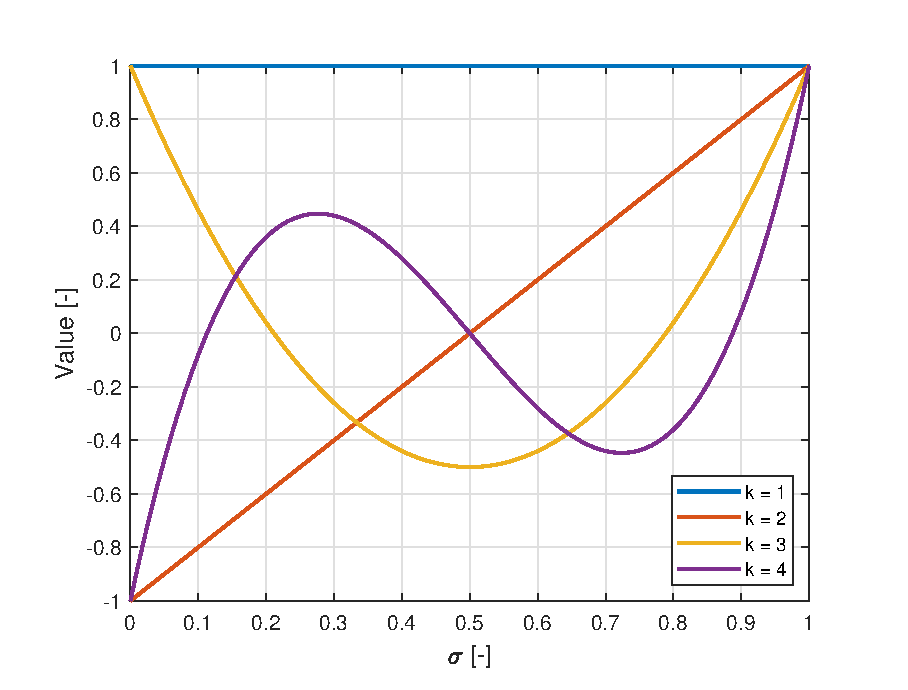
\includegraphics[width = 0.7\textwidth ]{Figures/Chapter2/shapefunction.eps}
    \caption{First 4 Legendre shape functions on domain $[0 \hspace{4pt} 1]$.}
    \label{fig2:shapefunction}
\end{figure}

Above figure shows that for $k=1$ the resulting Legendre polynomial is equal to $1 \hspace{2pt} \forall \sigma$. Furthermore, the figure shows that each degree of shape-function takes more complex shapes. Therefore increasing the order of shape functions allows the model to describe more complex robot configurations. To avoid coupling between the states, these shape functions must be orthogonal to each other. This means that $\int_\mathbb{X} \varphi_i \varphi_j d \sigma = 0$ for any $i \neq j$ and non-zero otherwise. The strain approximation of \ref{eq2:strainapprox} can be written as a $N$-th order expansion as,



\begin{equation}
\begin{aligned}
    \begin{bmatrix}\xi(\sigma,t)\end{bmatrix}_N = & \hspace{5pt}  (B_a \otimes [ \varphi_1(\sigma) \dots \varphi_N(\sigma) ])q(t) + \xi_0 \\ = &  \underbrace{ \begin{bmatrix}
    \varphi_1(\sigma) & \dots  & \varphi_N(\sigma) & \dots     & 0      & \dots  &  0 \\
    \vdots    & \ddots & \vdots    & \ddots    & \vdots & \ddots & \vdots \\
    0         & \dots  & 0         & \dots     & \varphi_1(\sigma) & \dots & \varphi_N (\sigma)
    \end{bmatrix}}_{\Phi(\sigma)} \begin{bmatrix} q_{1,1}(t) \\ \vdots \\ q_{3,N}(t) \end{bmatrix} +  \begin{bmatrix} \xi_{1,0} \\ \vdots \\ \xi_{3,0}   \end{bmatrix}
    \end{aligned},
\label{eq2:xishape}
\end{equation}

where $\Phi(\sigma) \in \mathbb{R}^{3 \times mN}$ is the Kronecker-product between matrix $B_a \subseteq \text{span} \hspace{2pt} I_3$ and transposed vector $\varphi(\sigma) \in \mathbb{R}^N$. Integer $m$ is defined as the number of active strains in the system. In this context, the active strains are strains that can be actively controlled. For our soft robot, this is the curvature $\kappa$ and the vertical elongation $\epsilon_y$. Hence, $m=2$ for our system. Based on these active strains, selection matrix of unconstrained strains can be defined as,

\begin{equation}
    B_a = \begin{bmatrix}
    1 & 0 \\
    0 & 0  \\
    0 & 1  \\
    \end{bmatrix}.
    \label{eq2:Ba}
\end{equation}

The entries of selection matrix $B_a$ tells that only the first and third strain are free. This also implies that only these two strains are approximated. At this point, we have presented the forward kinematic problem and showed the Galerkin reduction method to approximate strains. This approximation allows formulating the system in finite-dimension. Therefore, another assumption is made regarding the maximum truncation $N$ in our strain approximation.

\begin{theorem}
The strains induced by actuating the soft robot under basic operating conditions can be captured by truncation of $N = 1$. 
\end{theorem}

Based on this assumption, and the shape function polynomials of (\ref{eq2:shapefunction}) a first order approximation of the strains is made. Substitution of the provided expressions for $B_a$ (\ref{eq2:Ba}) and $\xi_0$ into (\ref{eq2:xishape}) the strains of the soft actuator can be described by,


\begin{equation}
    \begin{bmatrix}\xi(t)\end{bmatrix}_1 =\underbrace{B_a \otimes [\varphi_1]}_{\Phi(\sigma)} q(t) + \xi_0  =  \underbrace{\begin{bmatrix}
    1 & 0  \\
    0 & 0  \\
    0 & 1
    \end{bmatrix}}_{\Phi} \begin{bmatrix} q_{1,1}(t) \\  q_{2,1}(t) \end{bmatrix} +  \begin{bmatrix} 0 \\ 0 \\ 1   \end{bmatrix},
\label{eq2:xiapprox}
\end{equation}

where we can conclude that the approximated strain becomes space-invariant. For a first-order truncation the shape function is equal to $1 \hspace{2pt} \forall \sigma$, as is shown in Figure \ref{eq2:shapefunction}. Therefore, the Kronecker product between $B_a$ and $[\varphi_1]$ results in a space-invariant matrix $\Phi$ which has the same entries and structure as $B_a$. Furthermore, it can be seen that the second component of strain vector $[\xi(\sigma,t)]_1$, corresponding to elongation $\epsilon_x = 0 \hspace{3pt} \forall \hspace{3pt} \sigma $ and $ \forall \hspace{3pt} t$. This allows us to define the modal coordinate vector as,


\begin{equation}
q(t) = \begin{bmatrix} q_{1,1}(t) \\ q_{2,1}(t) \end{bmatrix} = \begin{bmatrix} \kappa(t) \\ \epsilon_y(t) \end{bmatrix} = \begin{bmatrix} \kappa(t) \\ \epsilon(t) \end{bmatrix}.
\end{equation}

Since there is zero strain in the x-direction, we will agree upon a new notation for the strains. Throughout this work, we will use ``elongation" or $\epsilon$ to address strain $\epsilon_y$. Likewise, ``curvature'', ``rotation'' or  $\kappa$ are used interchangeably to refer to curvature $\kappa$. Approximating strains and curvatures with a single shape function will reduce this Cosserat model to the piece-wise constant curvature (PCC) model as discussed in Chapter \ref{chapter1}. As can be seen from (\ref{eq2:shapefunction}), all shape functions yield 1 for $k=1$. In this case, the modal coordinates $q(t)$ will be equal to $\kappa$ and $\epsilon$, respectively. From this point onward, only a single shape function is used to approximate the strains and curvatures of the actuator. 

In the next section, the forward kinematic problem is solved with the described strain approximation.




\section{Forward kinematics}

The forward kinematic problem of (\ref{eq2:dgdsigma}) for the
planar soft robot is solved by spatial integration over domain $[0,L]$. At each discrete increment the strain field $[\xi(t)]_1$ is approximated by (\ref{eq2:xiapprox}). A standard ODE solver such as $\verb+ode45.m+$ in \MATLAB \cite{MATLAB2020} will suffice. The chosen initial condition is $g(0,t) = I_3 \hspace{2pt} \forall t$, which corresponds to zero rotation and zero strain at $\sigma = 0$. Furthermore, the chosen modal coordinates are constant as $q = q(t) \hspace{2pt} \forall t$. 

Figure \ref{fig1:forward_kinematic} shows the result of the forward kinematic model. The initial position is obtained for zero curvature and elongation. It can be seen that the undeformed length of the soft robot $L$ is equal to 64.5 mm. To obtain the deformed modal coordinate $q(t)$ was chosen equal to $[-17,0.1]^\top$. Physically this implies a clockwise rotation, creating an arc with a curvature of $18.7 \frac{1}{m}$, as the soft robot elongates by 10\%.


\begin{figure}[H]
    \centering
    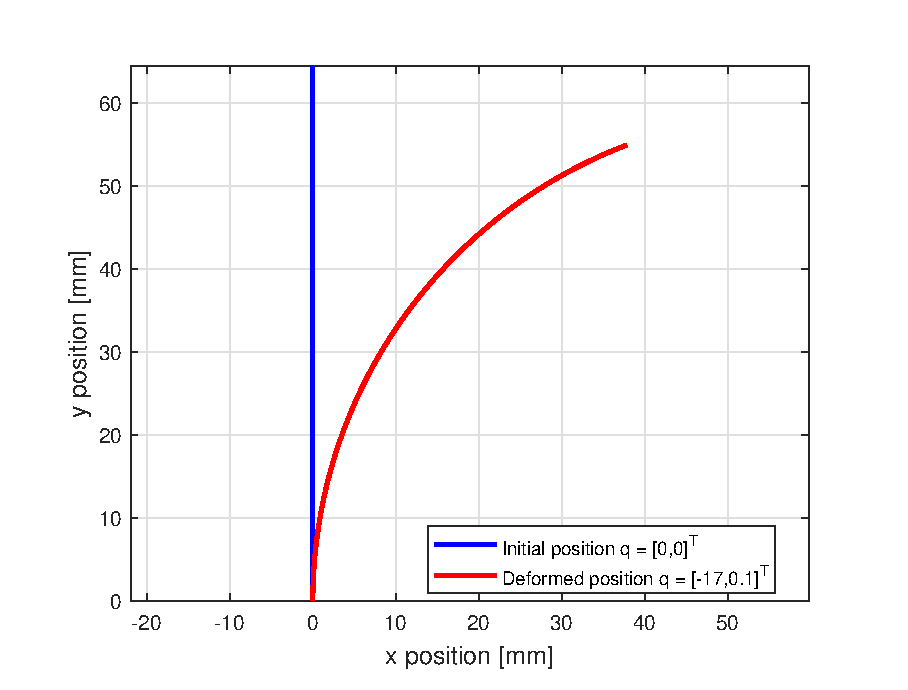
\includegraphics[width = 0.7\textwidth]{Figures/Chapter2/fkin1701.eps}
    \caption{Initial position and deformed position for a first order shape function approximation of the kinematic model.}
    \label{fig1:forward_kinematic}
\end{figure}

Besides a forward kinematic model, a numerical inverse kinematic solver was programmed. This allows defining a position in planar Cartesian coordinates, and obtain modal coordinates. The algorithm will minimize the distance between the desired end-effector position and reachable end-effector position given the number of truncations $N$. It shows the model's flexibility when using multiple shape functions. The algorithm is further detailed in Appendix \ref{app:chap2}. 

For now, we have neglected the time dependency of modal coordinate vector $q(t)$. To determine the dynamics of the system it is crucial to consider the time variance of the system as well. To do so, we first consider the velocity kinematics of the system in the next section.


\section{Velocity kinematics}

The velocity kinematics allows us to study velocities along the backbone curve. Similar to the spatial derivative, backbone curve $g(\sigma,t)$ can be differentiated with respect to time. This differentiation results in, 

\begin{equation}
  \Dot{g} = \frac{\partial g}{\partial t} = g \hat{\eta} \hspace{10pt} \implies \hspace{10pt}  \hat{\eta}(\sigma,t) := g^{-1}\dot{g} = \begin{bmatrix} 0 & -\omega & v_x \\ \omega & 0 & v_y \\
  0& 0 & 0 \end{bmatrix} \in  \mathfrak{se}(2)
    \label{eq2:dgdt}
\end{equation}

which describes the time-twist field in a local frame at $\sigma$ at time $t$. Since a planar case is considered, there is a single angular velocity. This curvature is expressed by a $2 \times 2$ skew-symmetric matrix obtained by $\frac{d}{dt}R(\sigma,t)R^\top(\sigma,t) \in \mathfrak{so}(2)$. Vector $V = [v_x,v_y]^\top \in \mathbb{R}^2$ contains linear velocities in perpendicular and tangential direction, respectively. Therefore, $\hat{\eta} \in \mathfrak{se}(2)$ effectively contains angular and linear velocities among the backbone curve. Due to the isomorphism of $\mathfrak{se}(2) \longmapsto \mathbb{R}^3$, all velocities can equivalently be stored in column vector $\eta(\sigma,t) := [\omega \hspace{3pt} v_x \hspace{3pt} v_y]^\top \in \mathbb{R}^3 \cong \mathfrak{se}(2)$ \cite{Sola2018}.


Using the equality of mixed partial derivatives, at each instant of space and time $\frac{\partial}{\partial t}g' = \frac{\partial}{\partial \sigma}\dot{g}$ holds \cite{Caasenbrood2020}. By using general rules of substitution and actions in Lie space it can be proven that the spatial derivative of the velocity field can be written as,

\begin{equation}
    \eta'(\sigma,t)= (\text{Ad}_{g(\sigma,t)^{-1}})'\text{Ad}_{g(\sigma,t)} \eta(\sigma,t) + \Dot{\xi}(\sigma,t) \hspace{10pt} \text{with} \hspace{10pt} \text{Ad}_{g(\sigma,t)} = \begin{bmatrix} 0_2^\top & 1 \\ \Tilde{s}(\sigma,t) & R(\sigma,t)  \end{bmatrix} \in \mathbb{R}^{3\times 3}
    \label{eq2:etadif}
\end{equation}


where $\text{Ad}_g \in \mathbb{R}^{3 \times 3}$ \cite{2DLie} is the adjoint mapping of $g$ \cite{Sola2018}. Vector $\Tilde{s}$ is defined as $[s_2(\sigma,t) \hspace{5pt} -s_1(\sigma,t)]^\top$ \cite{2DLie}, which can be derived from the adjoint action defined for the Lie group $\mathbb{SE}(3)$. This adjoint mapping allows velocities expressed in local frame $g(\sigma,t)$ to be mapped to frame $g(0,t)$, which coincides with our Cartesian coordinate frame. The complete derivation of (\ref{eq2:etadif}) is presented in Appendix \ref{app:chap2}. 

An analytic solution to (\ref{eq2:etadif}) can be found by integrating the equation over spatial domain $[0,\sigma]$. It is given that the actuator is fixed at one end. Therefore the boundary conditions $\eta_0 = 0_{3}^\top$ and $g_0 = I_{3}$ can be imposed. This physically means that at $\sigma = 0$ there is no velocity, strain nor curvature. Integrating over domain $[0,\sigma]$ will give accordingly,

\begin{equation}
  \begin{bmatrix} \eta(\sigma,t)\end{bmatrix}_1 = \text{Ad}_{[g(\sigma,t)]_1^{-1}} \int_0^{\sigma} \text{Ad}_{[g(\sigma,t)]_1} \Phi \hspace{2pt} d \sigma  \hspace{2pt} \dot{q}(t) = [J(\sigma,t)]_1\dot{q}(t),
    \label{eq2:J}
\end{equation}

here an expression for the geometric Jacobian $[J(\sigma,t)]_1 \in \mathbb{R}^{3\times 2}$ is obtained \cite{Caasenbrood2020}, for a first-order strain truncation. This Jacobian maps modal coordinate velocity to linear and angular velocities along the backbone curve. Recall that two active degrees of freedom are considered, that are strain $\epsilon$ in the y-direction and curvature strain $\kappa$. Therefore, the modal coordinate vector $q(t)$ is of dimension two. The geometric Jacobian maps the modal coordinate velocity $\dot{q}(t)$ to velocities in the Euclidean space. The velocity of a point with respect to a reference in 2-dimensional Euclidean space is described by 3 components. From our fixed reference point at $g(0,t)$, these velocities are one angular velocity, and two linear velocities in horizontal en vertical direction, respectively. This explains the dimension of the Jacobian matrix. As can be seen, this Jacobian matrix is non-linear with respect to space and time. Besides relating modal coordinate velocity to Cartesian velocity, the Jacobian can be used on position level as,

\begin{equation}
    r(\sigma,t) = [J(\sigma,t))]_1q(t),
\end{equation}

which implies that modal coordinates $q(t)$ can also be mapped to a position vector $r\in \mathbb{R}^3$ in Euclidean space. This position vector contains rotation, horizontal and vertical position as $[\theta \hspace{3pt} x \hspace{3pt} y]^\top$, respectively. Therefore this Jacobian is of valuable use for further system analysis. It can for instance be used in path-planning, as the Jacobian inverse can map Cartesian coordinates to modal coordinates. Furthermore, it can be used in controller design. However, in the next section, the Jacobian will be used for deriving the dynamics of the soft robot. 


\section{Dynamic model derivation}






To study the dynamic behaviour of the soft actuator a dynamic model is derived. A relatively simple approximation is used to obtain insight into the basic dynamics of the actuator. The dynamic model will primarily be used for controller design. A relatively simple model is deemed to be sufficient to assess general controller performance. We consider the following system of equations,

\begin{equation}
    \dot{x}_1  = f(x_1) + g(x_2) 
       \label{eq2:nonlineq1}
    \end{equation}
    \begin{equation}
    \dot{x}_2 = Ax_2 + Bu(t)  
    \label{eq2:nonlineq2}
\end{equation}

where $(\ref{eq2:nonlineq1})$ describes the soft robot dynamics and $(\ref{eq2:nonlineq2})$ the actuator dynamics. State vector $x_1$ is defined as $[ q \hspace{4pt} \dot{q} ]^\top$ corresponding to modal coordinate position and velocity. Function $f(x_1)$ is a nonlinear function representing the soft robot dynamics, dependent on $x_1$. Function $g(x_2)$ is the input function of the soft robot, which is dependent on state $x_2$. State vector $x_2$ is defined as $[ p_1 \hspace{4pt} p_2 ]^\top$, representing the individual bellow pressures. The actuator dynamics, that are air-pumps, are described by linear system matrix $A$. The control input matrix $B$ is multiplied by input function $u(t)$.

To model the soft robot dynamics the following assumption is made:

\begin{theorem}
The soft robot's dynamics can be modelled as a non-linear mass-spring-damper system, assuming that the system is negligibly affected by Coriolis effects. Gravitational effects are deemed insignificant due to the low system mass.
\end{theorem}

Neglecting the influence of gravity is deemed valid, as the mass of the system is very low ($m << 0.1 kg$). Given the system's low mass, and slow operating velocity, the contribution of the Coriolis terms are small. This Coriolis matrix contains terms $\dot{q}_i q_j$ with $i \neq j$. For low velocities, these cross-terms are deemed small. Therefore, the dynamic model will take the following structure,


\begin{equation}
    M(q)\Ddot{q} + D\dot{q} + K(q)q = \nu(p),
    \label{eq2:simp_model}
\end{equation}


where $M(q)$ is the non-linear mass matrix. Since the Jacobian matrix is position variant, it is assumed that the mass matrix will be position variant too. This makes the system non-linear. Furthermore, $D$ is a matrix corresponding to linear damping. Matrix $K(q)$ captures the non-linear stiffness. It is known that the elastomer of which the soft robot is composed deforms non-linearly. The input of the system is $\nu(p) \in \mathbb{R}^2$. This input vector consists of a moment and force that act on the system. 

The dynamic model as posed in (\ref{eq2:simp_model}) can be obtained based on Lagrangian method. The Lagrangian is defined as $\mathcal{L} = \mathcal{T} -\mathcal{V}$ which expresses the energy difference between kinetic energy $\mathcal{T}$ and potential energy $\mathcal{V}$. Exact expressions for the kinetic energy and potential energy of the system are given by, respectively,

\begin{equation}
    \mathcal{T} = \frac{1}{2}\int_0^{\sigma} \eta(\sigma,t)^\top \mathcal{M} \eta(\sigma,t) \hspace{2pt} ds \hspace{20pt} \text{and} \hspace{20pt}  \mathcal{V} = \frac{1}{2}\int_0^{\sigma} \xi(\sigma,t)^\top \mathcal{K} \xi(\sigma,t)  \hspace{2pt} ds,
    \label{eq2:T}
\end{equation}


where $\mathcal{M} \in \mathbb{R}^{3\times3}$ and $\mathcal{K} \in \mathbb{R}^{3\times3}$ are a diagonal mass tensor and stiffness tensor, respectively. The approximations for velocity (\ref{eq2:J}) and strain (\ref{eq2:xishape}) can be substituted in this equation to formulate the kinetic and potential energy as follows,

\begin{equation}
    \mathcal{T} = \frac{1}{2}\int_0^{\sigma} \Big([J(\sigma,t)]_1\dot{q}\Big)^\top \mathcal{M} \Big([J(\sigma,t)]_1\dot{q}\Big) \hspace{2pt} ds
\end{equation}

\begin{equation}
\begin{split}
    \mathcal{V} &= \mathcal{V}(q) + \mathcal{V}_0  \\
                &=  \frac{1}{2}\int_0^{\sigma} \big(\Phi q\big)^\top \mathcal{K} \big(\Phi q\big) \hspace{2pt} ds +\frac{1}{2} \int_0^\sigma \xi_0^\top \mathcal{K} \xi_0  \hspace{2pt} ds .
\end{split}
\end{equation}

Above expression allows deriving the Lagrangian equations of motion as \cite{NWouw},

\begin{equation}
    \frac{\partial}{\partial t}\Big( \frac{\partial}{\partial\dot{q}}\mathcal{T}\Big)- \frac{\partial}{\partial q}\mathcal{T} + \frac{\partial}{\partial q}\mathcal{V} = \mathcal{Q}^{nc} \hspace{10pt} \text{with} \hspace{10pt} \mathcal{Q}^{nc} =  \nu(p) - \int_0^\sigma \big(\Phi\dot{q}\big)^\top \mathcal{D} \big( \Phi \dot{q}\big) \hspace{2pt} d \sigma
    \label{eq2:lagrange}
\end{equation}

where $\mathcal{Q}^{nc} \in \mathbb{R}^3$ is a vector containing non-conservative forces acting on the system. One of these non-conservative forces are actuation forces. These actuation forces are captured in vector $\nu(p) \in \mathbb{R}^2$. Another non-conservative force are the damping forces as a result of the energy dissipation in the elastomer. These damping terms are captured in diagonal damping tensor $\mathcal{D} \in \mathbb{R}^{3 \times 3}$. Also note that we have substituted the approximated strain rate which, without further prove, can be easily obtained from (\ref{eq2:xiapprox}). Further working out (\ref{eq2:lagrange}) and rearranging terms gives,

\begin{equation}
    \int_0^\sigma \Big( \underbrace{[J(\sigma,t)]_1^\top \mathcal{M} [J(\sigma,t)]_1}_{M(q)} \ddot{q}(t) +  \underbrace{\Phi^\top \mathcal{D} \Phi }_{D} \dot{q}(t)    +   \underbrace{\Phi^\top \mathcal{K} \Phi}_{K(q)} q(t)\Big) \hspace{2pt} d\sigma = \nu(p),
\end{equation}

here it becomes clear that $M(q)$, $D(q)$ and $K(q)$ are all in $\mathbb{R}^{2\times2}$, since $[J(\sigma,t)]_1 \land \Phi \in \mathbb{R}^{3 \times 2}$. Since we have assumed that the Coriolis effects are small, the term $\frac{\partial}{\partial q}\mathcal{T} \approx O_2 $ is omitted. Now the expressions for the mass, damping and stiffness matrices are presented, we will elucidate on the entries of their tensors, respectively.

In our modelling approach, the actuator kinematics have been described by a one-dimensional backbone curve. To derive the mass matrix, mass properties need to be assigned to this curve. Therefore the backbone curve is discretized, and we consider an infinitely thin slice of the cross-section of the actuator. To derive the mass tensor of the system the following assumption is made.

\begin{theorem}
The inertial properties of the actuator can be determined by considering an infinitely thin slice in the transverse direction and regarding it as a solid cuboid, which is independent of the state $q$ or $\sigma$.
\end{theorem}

Figure (\ref{fig:massapprox}) shows such a discretized cross section. Here the blue marked area is a solid cuboid with height $h$, width $w$, density $\rho$ and slice thickness $d\sigma$. 


\begin{figure}[H]
    \centering
    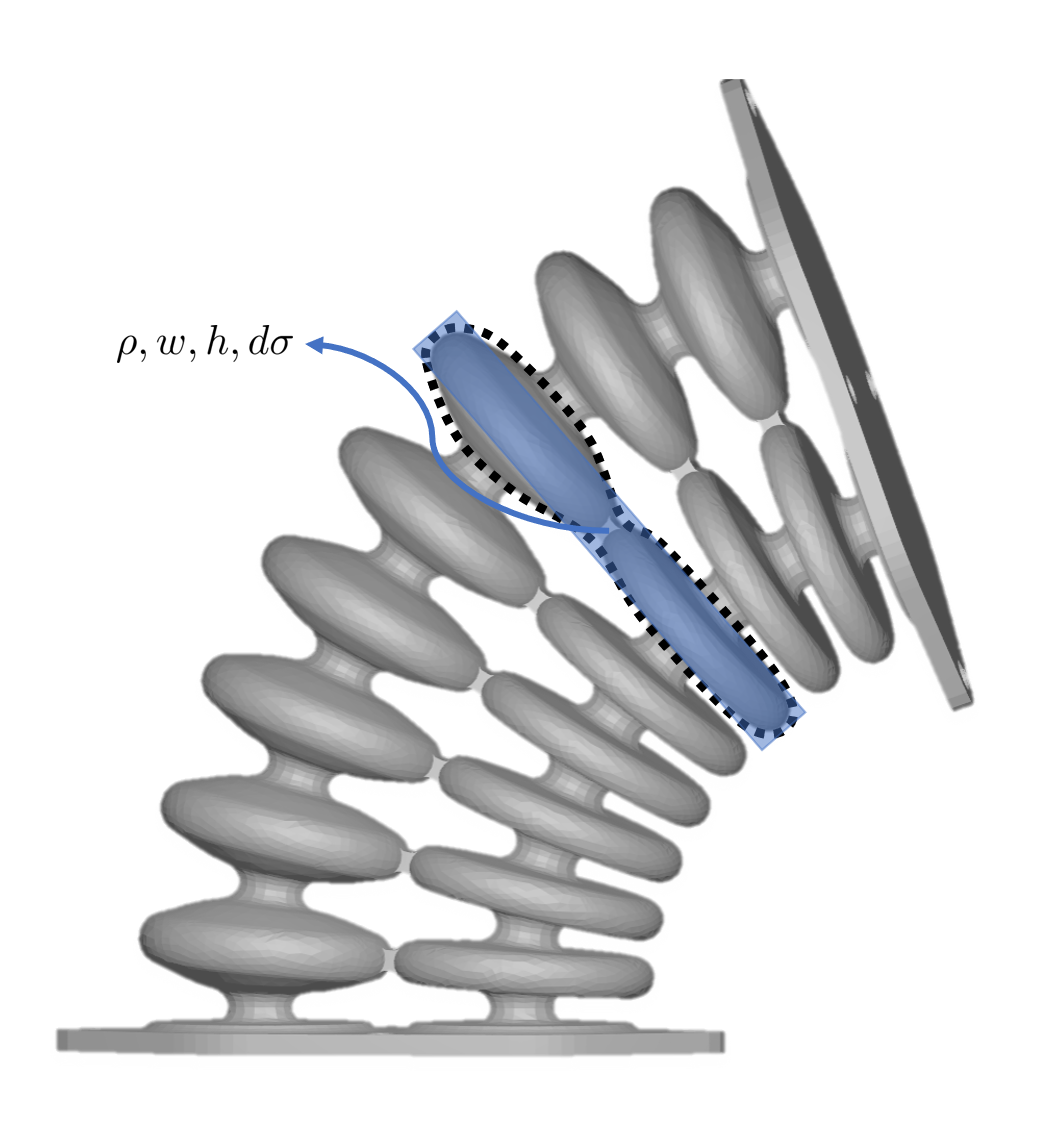
\includegraphics[width = 0.4\textwidth]{Figures/Chapter2/massapprox.png}
    \caption{Inertial properties can be determined by regarding an infinitely thin slice. The cross section is then viewed a solid cuboid.}
    \label{fig:massapprox}
\end{figure}


The mass tensor $\mathcal{M}$ then takes the following form,

\begin{equation}
    \mathcal{M} = \begin{bmatrix} \frac{1}{12}\rho w^2 & 0 & 0 \\
                                   0 & \rho & 0 \\
                                   0 & 0 & \rho \end{bmatrix}\hspace{5pt} \text{with} \hspace{5pt} \rho = \frac{m_{tot}}{L}
\end{equation} 




where $m_{tot}$ is the total mass of the actuator. The first entry expresses mass moments of inertia, related to the curvature acceleration of the actuator. The last two entries relate to the linear acceleration of the centre of mass of the cuboid. Based on equation (\ref{eq2:T}) the space-time variant mass matrix can be expressed as, 


\begin{equation}
    M(q)) = \int_0^{\sigma} [J(\sigma,t)]_1^\top \mathcal{M}(\sigma)[J(\sigma,t)]_1  \hspace{2pt}ds,
\end{equation}

here it should be noted this mass-matrix has off-diagonal entries related to the non-linear Jacobian matrix. 

We assume that the polymer of which the actuator is made has linear damping characteristics, therefore the damping matrix is space-time invariant and can be presented as,

\begin{equation}
    D = \int_0^\sigma \Phi^\top \mathcal{D} \Phi \hspace{2pt} ds  := \text{diag}([D_\kappa, D_\epsilon]),
\end{equation}

which has no off-diagonal terms. Effectively, this means that we are trying to find damping parameters $D_\kappa$ and $D_\epsilon$ related to curvature velocity and strain rate, respectively. These damping parameters will be chosen iteratively, as it is impossible to measure damping properties experimentally. The system can not be actuated such that a single degree of freedom is excited. 

It is given that the polymer has non-linear stiffness properties, which implies that stiffness matrix $K(q(t))$ is space-variant. The stiffness matrix is described as,

\begin{equation}
    K(q) = \int_0^\sigma \Phi^\top \mathcal{K}(q) \Phi \hspace{2pt} ds := \text{diag}([K_\kappa(q), K_\epsilon(q)]),
\end{equation}

which has no off-diagonal terms. Essentially, this means that only curvature stiffness $K_\kappa(q)$ and elongation stiffness $K_\epsilon(q)$ need to be determined. The process of obtaining these non-linear stuffiness's is explained in Chapter \ref{chap3}. Furthermore, the geometric properties and material properties are presented needed to compute the mass tensor. Up until now we have neglected the input function $\nu(p)$. This input vector will also be obtained in Chapter \ref{chap3}. 




\section{Pump model}

At this point, we have derived a dynamic model for our soft robot. However, actuation plays a dominant role in controlling our soft robot. Therefore it important to include pressure dynamics as well. Each bellow of the soft robot is pressurized using a diaphragm air pump. These air pumps compress air using membranes. The speed at which the membranes open and close determines the rate at which pressure increases. This speed can be regulated by supplying a DC voltage to the electric motor which opens and closes the membranes. To model the air pumps dynamics we make the following assumption.

\begin{theorem}
The air pumps used for actuating the soft robot have identical dynamics that can be described by a first-order model.
\end{theorem}

This assumption allows to formulate the pump dynamics as,

\begin{equation}
 \underbrace{\dot{p}}_{\dot{x_2}}  = \underbrace{\begin{bmatrix} -\lambda_1 & 0 \\ 0 & -\lambda_1 \end{bmatrix} p}_{Ax_2} + \underbrace{\begin{bmatrix} \lambda_2 & 0 \\ 0 & \lambda_2 \end{bmatrix} V(t)}_{Bu(t)},
    \label{eq2:pumpmodel}
\end{equation}

where $p =  [p_1 \hspace{4pt} p_2]^\top$ is the pressure based on input DC-voltage $V(t)$. The structure of (\ref{eq2:nonlineq2}) can already be observed in which $x_2 = p$. Constant $\lambda_1 \in \mathbb{R}^+$ represents the system's resistance to a pressure increase and is dependent on actual system pressure. Parameter $\lambda_2 \in \mathbb{R}^+$ is a constant that incorporates the pressure increase relative to the volt input signal. Additionally, it should be noted that this $\lambda_1$ acts as some deflation coefficient. For zero volt input, the system pressure decreases with a rate relative to the system pressure. This is captured by this pump parameter. Both of these parameters can be obtained via experimental analysis. This process is detailed in Chapter \ref{chap3}.







\section{Overall system dynamics}


In order to numerically solve the dynamic model,  (\ref{eq2:simp_model}) is reformulated to a second order state-space formulation as,

\begin{equation}
    \underbrace{\begin{bmatrix}\dot{q}\\ \ddot{q}  \end{bmatrix}}_{\dot{x}_1}   = \underbrace{  \begin{bmatrix} O_{2} & I_{2} \\ -M(q)^{-1}K(q)  & -M(q)^{-1} D \end{bmatrix}   \begin{bmatrix} q \\ \dot{q} \end{bmatrix} }_{f(x_1)}  +      \underbrace{ \begin{bmatrix} O_{2} \\ M(q)^{-1}   \end{bmatrix}       \begin{bmatrix} \nu_1(p) \\ \nu_2(p)  
    \end{bmatrix} }_{g(x_2)}, 
    \label{eq4:SS}
\end{equation}

where the structure of (\ref{eq2:nonlineq1}) can be recognized. State vector $x_1 = [ q \hspace{3pt} \dot{q}   ]^\top =  [\kappa \hspace{3pt} \epsilon \hspace{3pt} \dot{\kappa}  \hspace{3pt} \dot{\epsilon}  ]^{\top}$ and $x_2 = p$. From a physical standpoint the entries of the input vector $\nu$ can interpreted as a moment and a force acting on the system. This moment $\nu_1$ causes the actuator to curve, whereas $\nu_2$ can be viewed as a force that causes elongation.


The system of equations as presented in (\ref{eq2:nonlineq1}) and (\ref{eq2:nonlineq2}) can be combined to capture the overall system dynamics. To do so, the state vector is defined as $x = [x_1 \hspace{4pt} x_2]^\top$. Furthermore, the input $\nu(p)$ should be related to pressure. Hereto a linear mapping is proposed as $\nu(p) = H p$, where $H \in \mathbb{R}^{2\times 2}$ maps pressure vector $p$ to input moment and force. 

Combining the soft robot dynamics of the provided state-space model in (\ref{eq4:SS}) with the pump model of (\ref{eq2:pumpmodel}). The overall dynamics can be captured by the following state space representation,

\begin{equation}
     \begin{bmatrix} \dot{x}  \end{bmatrix}   =   \underbrace{ \begin{bmatrix} O_{2\times 2} & I_{2} & O_{2} \\ -M(q)^{-1}K(q)  & -M(q)^{-1} D & O_{2} \\
     O_{2} & O_{2}    & -\lambda_1 I_{2}\ \end{bmatrix}   }_A   \begin{bmatrix} x \end{bmatrix}  + \underbrace{      \begin{bmatrix} O_{2} & O_{2} \\ M(q)^{-1}H & O_{2} \\ O_{2} & \lambda_2 I_{2} \end{bmatrix} }_B      \begin{bmatrix} p_1 \\ p_2  \\ V_1 \\ V_2 \end{bmatrix},
     \label{eq:ssp}
\end{equation}

where matrix $A \in \mathbb{R}^{6\times 6}$ contains the complete system dynamics and matrix $B \in \mathbb{R}^{6\times 4}$ contains the control input. Also note the substitution of $\nu(p) = Hp$.



\section*{Summary}

In this chapter, a dynamic model for the entire system is deduced. Based on the Cosserat beam model a continuous backbone curve was formulated along the centre of the soft robot. This backbone curve is a function of space and time. Differentiating this curve with respect to space allows deriving the forward kinematics. The time derivative of the backbone curve is utilized to derive the Jacobian matrix. This Jacobian matrix allows mapping modal coordinates to Cartesian coordinates. The soft robot dynamics were captured using a non-linear mass-damper-damper model. Based on the Lagrangian method the mass, damping and stiffness matrices are derived. To model the pump dynamics, a first-order linear model is assumed. The dynamic model of the soft robot was combined with the pump model to create a state-space model. 

\cleardoublepage

\chapter{Parameter Identification}
\label{chap3}

This chapter details the parameter identification of the soft robotic actuator. First, material properties and dimensions of the soft robotic manipulator are provided. Then, determination of actuator stiffness for elongation and curvature explained. Consequently, pressure to force input mapping is detailed. At this point it should be emphasized that during experimental analysis the soft actuator, on which this parameter study is based, was too porous. This allowed too much air to escape and therefore was not suitable for further use. Therefore, the methodology of acquiring stiffness data and pressure mapping should be valued instead of found parameters. During experimental analysis a geometric equivalent planar actuator is used. 


Parameter identification is necessary for model simulation as well as experimental validation. Key actuator parameters such as actuator mass and dimensions were presented in an earlier work \cite{berkers}. Since the robotic manipulator is manufactured by an external company, some material properties are classified. To our best knowledge, the Young's Modulus and Poisson ratio are equal to those presented in Table (\ref{tab4:parameters}). These properties allow to calculate shear modulus $G$ as $\frac{E}{2(1+\nu)}$ and bulk modulus $K$ as $\frac{E}{3(1-2\nu)}$. It is assumed that the robotic manipulator deforms non-linearly following Neo-Hookeon behaviour \cite{Caasenbrood2020StiffnessModel}. For consistency with linear elasticity these moduli are reformulated as $C_{10} = \frac{\mu}{2}$ and $D_{1} = \frac{2}{\kappa}$ as used for Finite Element Analysis (FEA) \cite{neohookean}. The geometrical properties are presented in Figure \ref{fig3:dim}.


\begin{table}[H]
    \centering
    \caption{Actuator properties}
    \begin{tabular}{|c|c|c|} \hline
      \textbf{Parameter}   &  \textbf{Value} & \textbf{Unit} \\ \hline
      Mass $m$             &    0.0332       & $[kg]$ \\ 
      Nominal length $L_0$ &    0.0644       & $[m]$  \\ 
      Actuator width  $w$     &    0.0664       & $[m]$  \\
      Lever length $r$     &    0.01256      & $[m]$  \\ 
      Young's Modulus $E$  &    69           & $[MPa]$\\ 
      Poisson ratio $\nu$ &    0.45         & $[-]$ \\ \hline
    \end{tabular}
    \label{tab4:parameters}
\end{table}

\begin{figure}[H] 
    \begin{minipage}[b]{0.49\linewidth}
     \centering
    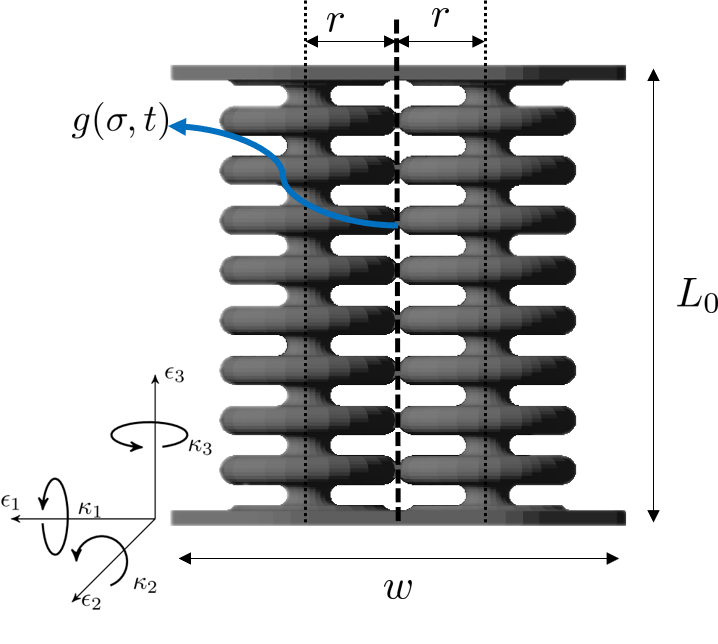
\includegraphics[width=\linewidth]{Figures/Chapter3/dimensions.png} 
    \caption{Schematic overview of the undeformed actuator with its dimensions.} 
    \label{fig3:dim} 
       \end{minipage} 
    \begin{minipage}[b]{0.49\linewidth}
     \centering
    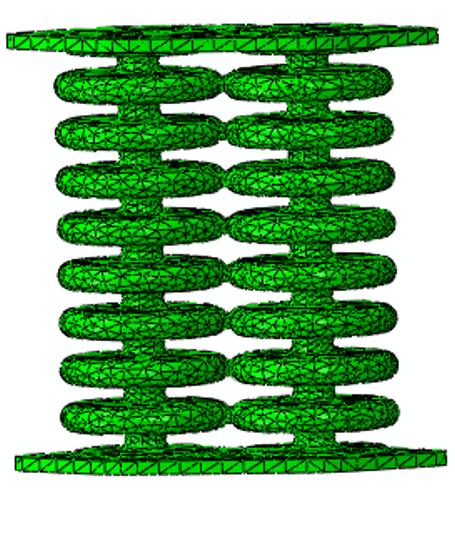
\includegraphics[width=0.7\linewidth]{Figures/Chapter3/undeformed2.png} 
    \caption{Undeformed meshed Finite Element model of the planar actuator.} 
    \label{fig3:FemModel} 
    \end{minipage} 
\end{figure}

%%%%%%%%%%%%%%%%%%%%%%%%%%%%%%%%%%%%%%%%%%%%%%%%%%%%%%%%%%%%%%%%%%%%%%%%
%%%%%%%%%%%%%%%%%%%%%%%%%%%%%%%%%%%%%%%%%%%%%%%%%%%%%%%%%%%%%%%%%%%%%%%%
%%%%%%%%%%%%%%%%%%%%%%%%%%%%%%%%%%%%%%%%%%%%%%%%%%%%%%%%%%%%%%%%%%%%%%%%

\section{Finite Element Analysis (FEA)}

In an effort to determine stiffness properties, finite element software \verb+Abaqus/CAE+ is used. This software allows to study deformation of the actuator under various loads. Stiffness can be approximated by relating applied forces to the magnitude of deformation. Here we want to relate pressure, thus its resulting force, to induced elongation and curvature. Figure  \ref{fig3:FemModel} shows the meshed model used in the finite element software. A mesh refinement analysis is done to determine an accurate mesh size, see Appendix \ref{app:chap3}. In the analysis, the bottom plate of the actuator is constrained in all directions of motion and rotation. Furthermore, the out-of-plane motion of the actuator is not considered since the body is symmetric, and applied loads act perpendicular to this motion. Also, gravitational effects are omitted. Lastly, the following assumption is made. 

\begin{theorem}
The actuator is assumed to be symmetrical along its longitudinal axis. Both bellows therefore deform uniformly.
\end{theorem}


In this finite element analysis we only consider the curvature induced by pressurizing a single bellow. Due to symmetry we assume that inflating the other bellow will result in equal rotation but in opposite direction. Two different analysis are performed. The first analysis focuses on curvature, the second analysis targets elongation. 


\subsection{Curvature analysis}

The curvature analysis allows to determine rotation stiffness of the robot manipulator. For this analysis only a single bellow is pressurized, while the other bellow pressure is kept zero. The force created by this pressurized bellow causes a moment around the center of the actuator. This will case the actuator to curve and elongate. Figure \ref{fig3:schematiccurvature} shows the deformation the actuator undergoes during a curvature simulation. Here the undeformed actuator is visualized in blue. For the black actuator the left bellow is pressurized to 60 kPa.


After applying loads to the finite element model, nodal displacements can be outputted from $\verb+Abaqus+$. The acquired data is post-processed in \MATLAB to estimate the elongation and curvature. A post-processed image of the deformation is shown in Figure \ref{fig3:nodalcurvatrue}. This image is created by isolating specific nodes, necessary to reconstruct the backbone curve. In this figure, top and bottom plate of the actuator are clearly visible. Using \MATLAB function \verb+affine_fit.m+ \cite{affinefit} the orientation of both planes with their normal vector can be obtained. Furthermore, this function determines the weighted average of all nodes of the top plate. Which coincides with the end-effector position of the actuator. Lastly, the nodes that are situated at the exact geometrical mid over the longitudinal axis are isolated. These clusters of nodes are used to reconstruct the backbone curve. 


The post-processed image can be used for kinematic model fitting. This is the last step to obtain modal coordinates $\epsilon$ and $\kappa$ from the finite element simulation. Figure \ref{fig3:nodalfitcurv} shows this kinematic model fit. Here the black cross again indicates the end-effector position. Initially, the kinematic fitting is done with the aid of the developed inverse kinematic model as detailed in Appendix \ref{app:chap2}. An inverse kinematic solution can be found based on the end-effector position and rotation. The solution to this kinematic fitting procedure is indicated by the purple curve. This result was deemed insufficiently accurate. Therefore an optimization method is proposed. This optimization method takes into account the curvature of the entire backbone curve. For each cluster of nodes among the backbone the weighted average is calculated. Those are indicated with a blue cross and denoted as vector $\Bar{x}_{mid} \in \mathbb{R}^{2\times N}$. Furthermore, the length of the backbone curve is determined using the function \verb+arc_length.m+ \cite{arclength}. This functions uses vector $\Bar{x}_{mid}$ to approximate the arc length using splines. This estimated arc length is represented as  $\Bar{x}_{length} \in \mathbb{R}^+ $. The optimization is done via optimization with \verb+fmincon.m+. The minimization problem that follows is,


\begin{equation}
\begin{aligned}
\min_{q} \hspace{5pt}  q^\top Q q  + \sum_{i=1}^{N}[\Phi_1(\Bar{x}_{mid} - f(q))^2] +   \Phi_2(\Bar{x}_{end}  - f(q)_{end})^2 +  \Phi_3(\Bar{x}_{length} - & f(q)_{length})^2  \\ 
\text{s.t.} \hspace{5pt} \epsilon - 1 > 0
\end{aligned}
\label{eq3:optim}
\end{equation}


where $f(q)$ is a function describing the forward kinematics based on modal coordinate vector $q$. Furthermore, $Q$ is $\text{diag}([0.001,0.001])$ is a weighing matrix used to penalize the value of the modal coordinates. Additional weighing factors $\Phi_i \in \mathbb{R}^+$ and $i \in \{1,2,3\}$ are applied to penalize individual terms and equal to $5e4$,$5e4$ and $1e4$, respectively. This weighing factors can used to scale individual error terms, and stress relative importance. The imposed constrained affects the elongation of the manipulator. Physically this constraint implies that the actuator can shorten in length, but the length can not become negative. As a note, for a single shape-function approximation, solving the minimization problem only results in little better modal coordinate estimates. For studying more complex actuator deformations, that involve estimations with multiple shape functions, this optimization is necessary. An inverse jacobian search singularly based on end-effector position will not be enough then. Some reconstruction of the backbone curve will be necessary for such cases. The modal coordinates belonging to the deformation of Figure \ref{fig3:nodalfitcurv} find through optimization for this simulation are $q = [\kappa,\epsilon]^\top = [-14,0.24]^\top$.




Above described inverse kinematic optimization is ran for multiple finite element analysis conducted various pressures. The results are displayed in Figure \ref{fig3:rotationvspressure}. Here the obtained curvature and elongation are plotted as a function of bellow pressure. It can be seen that the curvature and elongation rates increase by increments in pressure. Also the non-linear relation between pressure and deformation is visible.

\begin{figure}[H]
    \centering
\begin{minipage}{0.5\textwidth}
        \centering
        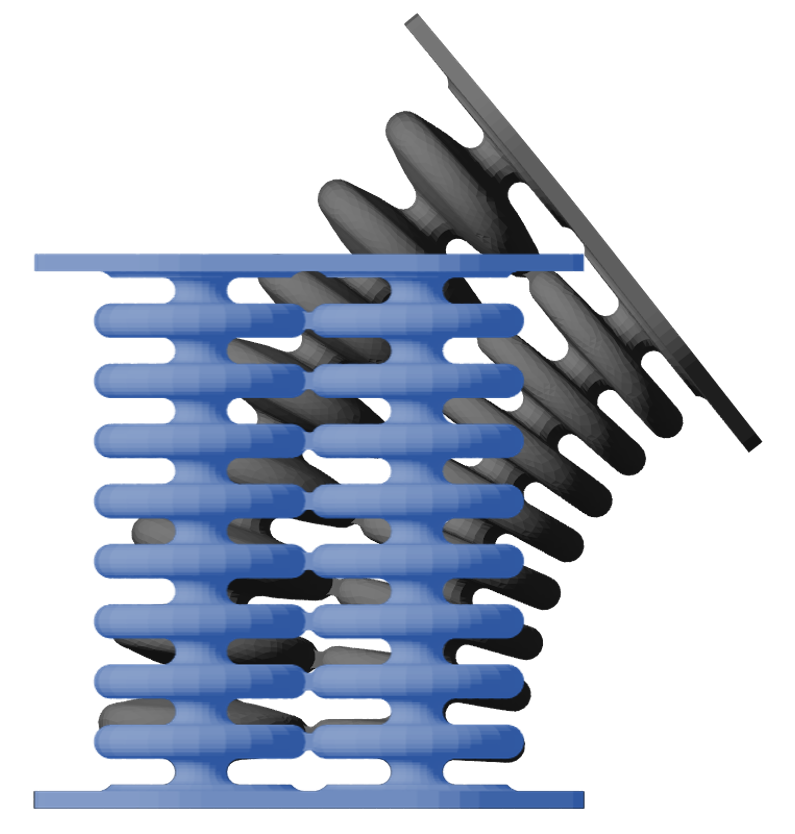
\includegraphics[width=0.695\textwidth]{Figures/Chapter3/curvature.png} 
        \caption{Curvature analysis, undeformed actuator blue and deformed actuator for curvature experiment. }
        \label{fig3:schematiccurvature}
    \end{minipage}\hfill
    \begin{minipage}{0.5\textwidth}
        \centering
        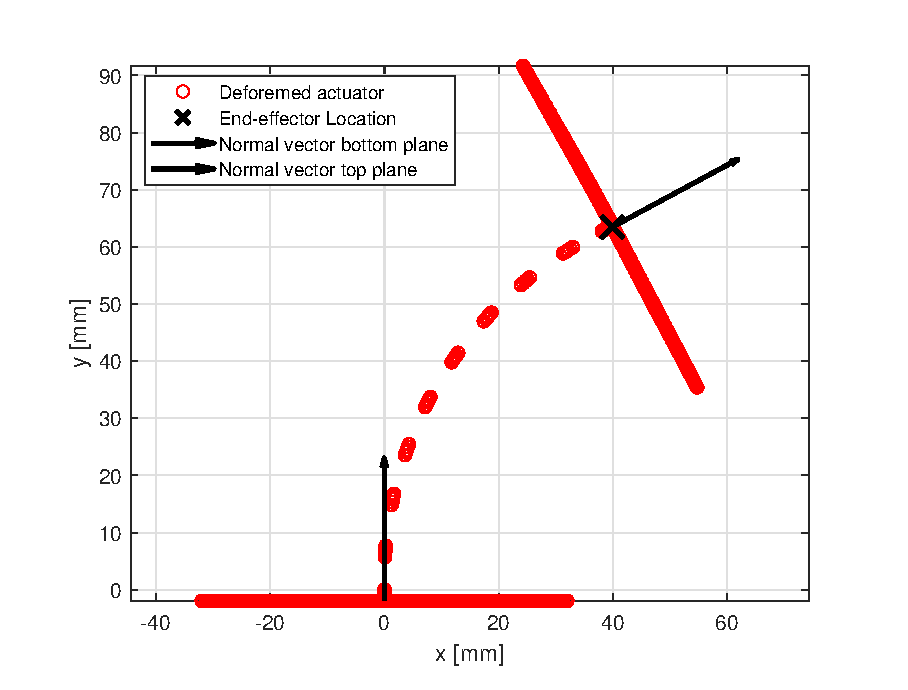
\includegraphics[width=\textwidth]{Figures/Chapter3/rotation60kpa.eps} 
        \caption{Post-processed image of the curvature analysis. The nodes that form the backbone curve clearly isolated.}
        \label{fig3:nodalcurvatrue}
    \end{minipage}
\begin{minipage}{0.5\textwidth}
        \centering
        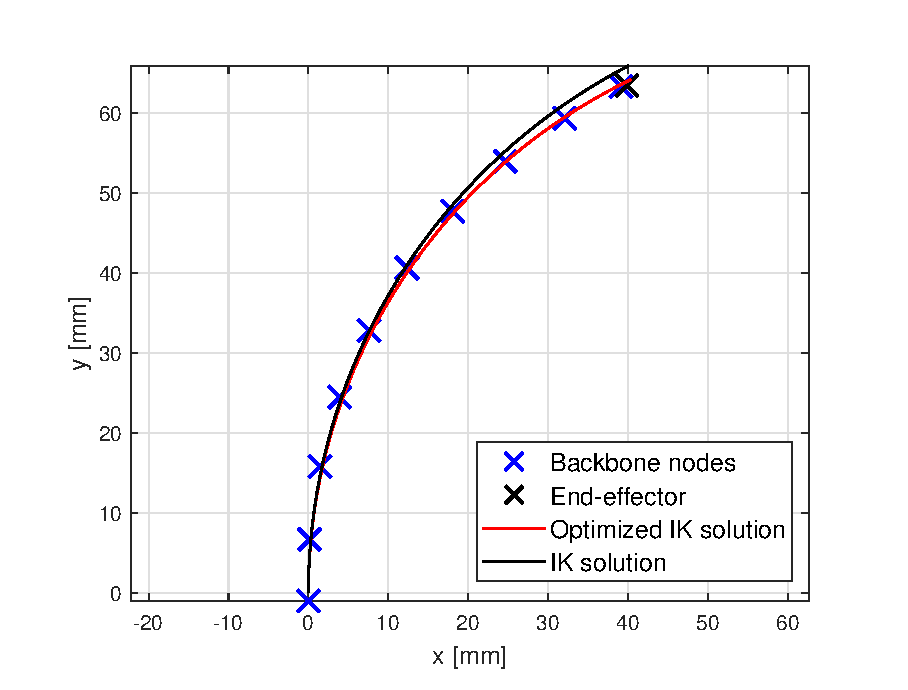
\includegraphics[width=\textwidth]{Figures/Chapter3/rot60kpa.eps}
        \caption{Inverse kinematic fit for an curvature analysis. Left bellow pressurized to 60kPa.}
        \label{fig3:nodalfitcurv}
    \end{minipage}\hfill
    \begin{minipage}{0.5\textwidth}
        \centering
        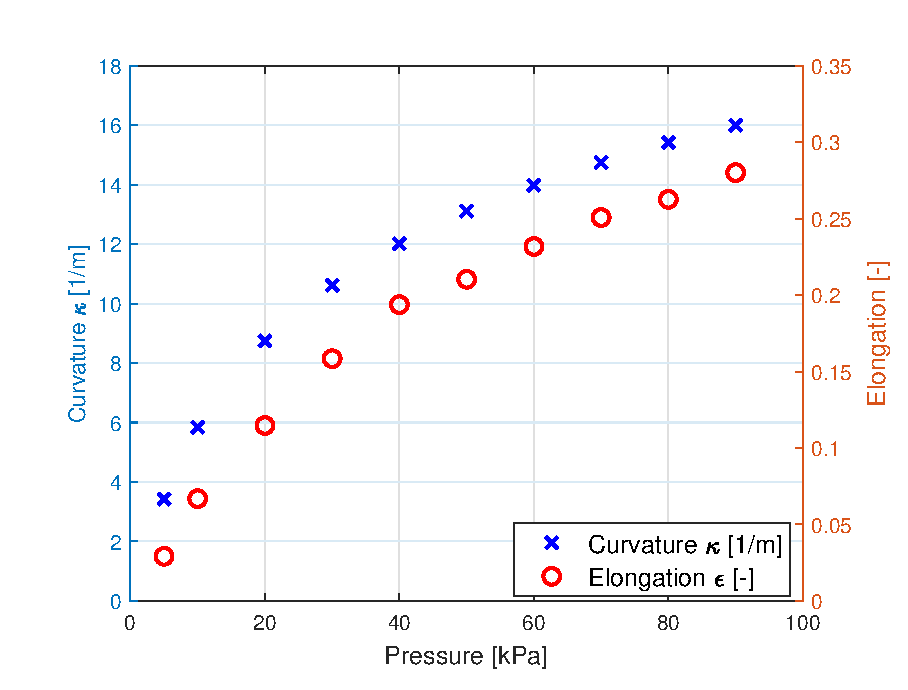
\includegraphics[width=\textwidth]{Figures/Chapter3/curvanalysiscurveps.eps} 
        \caption{Curvature analysis, elongation and curvature as function of pressure.}
        \label{fig3:rotationvspressure}
    \end{minipage}
\end{figure}

\newpage





\subsection{Elongation analysis}


The elongation analysis aims to measure pure elongation of the soft actuator. This allows for determining elongation stiffness, as rotating effects of the top of the robot are small. ``Pure'' elongation is induced by pressurizing both bellows equally. Figure \ref{fig3:schematicelong} shows the deformation the actuator undergoes during an elongation experiment. Here the undeformed actuator is visualized in blue. For the black actuator both bellows are pressurized to 60 kPa. 

As for the curvature analysis, a post-processed image of the deformation is shown in Figure \ref{fig3:nodalelong}. The optimization of (\ref{eq3:optim}) is carried out, to determine modal coordinates. The results of this optimization is shown in Figure \ref{fig3:nodalfitelong}. The modal coordinates belonging to this fit are  $q = [\kappa,\epsilon] = [0.06, 0.45]^\top$, showing a negligible curvature. Furthermore, this figure shows that for elongation analysis, the developed inverse kinematic algorithm (Appendix \ref{app:chap2}) already yields decent results.  

Repeating this experiment for a set of pressures, a relation between elongation and pressure can be found. Figure (\ref{fig3:elongationvspressure}) shows the relation between elongation function of pressure. Additionally, the curvature of the manipulator is shown for various pressures. It can be seen that pressurizing the bellows equally results in a near pure elongation. The maximum obtained curvature is equal to 0.07 [1/m], which is equivalent to a rotation of around 0.32 degrees. This allows to determine the elongation stiffness as effects of rotation are deemed negligible. The elongation rate decreases as pressure increases, this is the result of a non-linear material parameters. As a remark, the found elongation for the elongation analysis is about double to those found for curvature analysis. For instance, the found elongation for the elongation experiment at 90 kPa is $0.55$, whereas for the curvature analysis the elongation at this pressure is $0.27$. This observation tells that the curvature and elongation are largely decoupled.

\newpage



\begin{figure}[H]
    \centering
\begin{minipage}{0.5\textwidth}
        \centering
        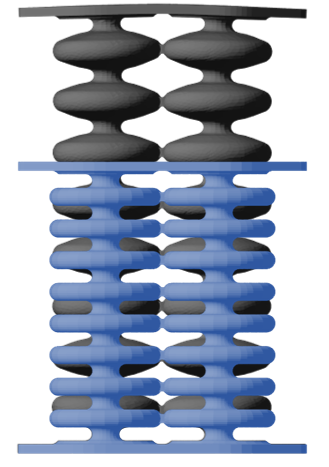
\includegraphics[width=0.53\textwidth]{Figures/Chapter3/elongation.png} 
        \caption{Elongation analysis, elongation and curvature as function of pressure. As can be seen curvature is negligibly small. }
        \label{fig3:schematicelong}
    \end{minipage}\hfill
    \begin{minipage}{0.5\textwidth}
        \centering
        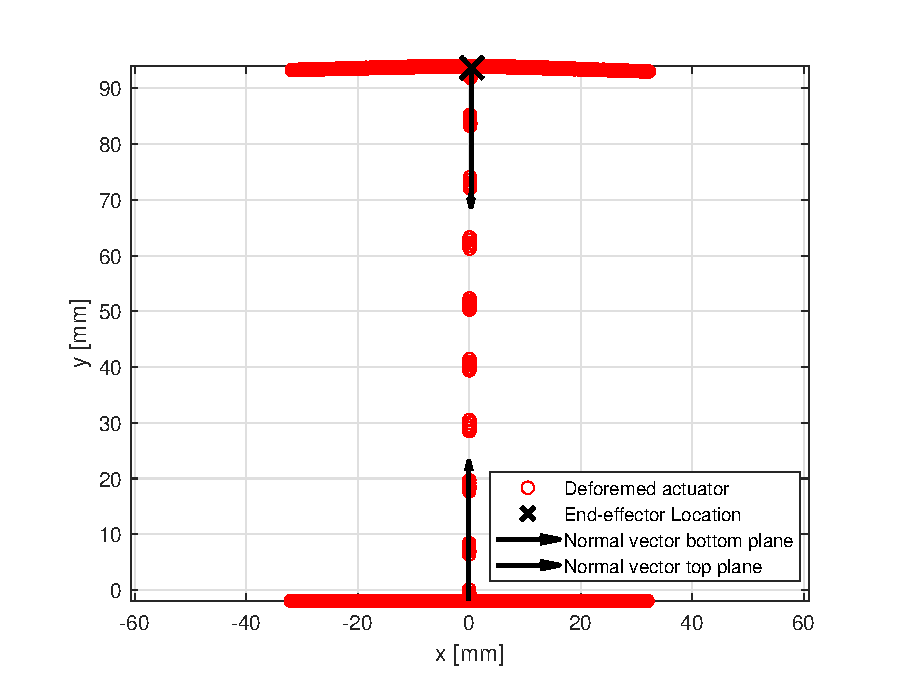
\includegraphics[width=\textwidth]{Figures/Chapter3/elongation60good.eps} 
        \caption{Post-processed image of an elongation analysis. The nodes that form the backbone curve clearly isolated.}
        \label{fig3:nodalelong}
    \end{minipage}
\begin{minipage}{0.5\textwidth}
        \centering
        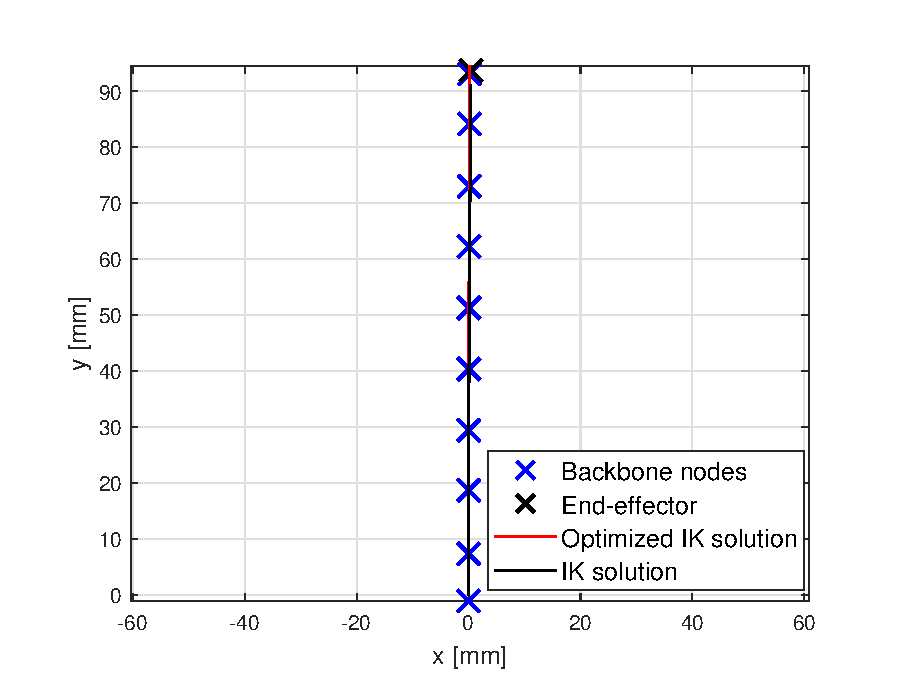
\includegraphics[width=\textwidth]{Figures/Chapter3/elong60kpa.eps}
        \caption{Inverse kinematic fit for an elongation analysis. Both bellows pressurized to 60kPa.}
        \label{fig3:nodalfitelong}
    \end{minipage}\hfill
    \begin{minipage}{0.5\textwidth}
        \centering
        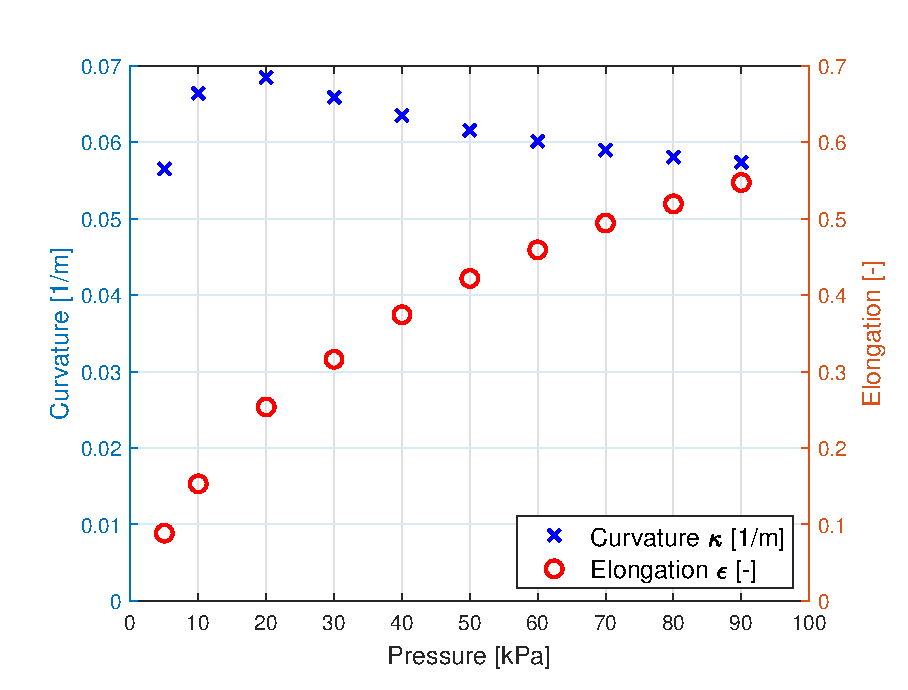
\includegraphics[width=\textwidth]{Figures/Chapter3/elonganalysiscurveps.eps} 
        \caption{Elongation analysis, elongation and curvature as function of pressure. As can be seen curvature is negligibly small.}
        \label{fig3:elongationvspressure}
    \end{minipage}
\end{figure}


At this point we have derived modal coordinates as function pressure. However, to determine the stiffness this pressure needs to be mapped to force and moment. This is discussed in Section \ref{sec3:InputMapping}.



%%%%%%%%%%%%%%%%%%%%%%%%%%%%%%%%%%%%%%%%%%%%%%%%%%%%%%%%%%%%%%%%%%%%%%%%
%%%%%%%%%%%%%%%%%%%%%%%%%%%%%%%%%%%%%%%%%%%%%%%%%%%%%%%%%%%%%%%%%%%%%%%%
%%%%%%%%%%%%%%%%%%%%%%%%%%%%%%%%%%%%%%%%%%%%%%%%%%%%%%%%%%%%%%%%%%%%%%%%



\section{Input Mapping}
\label{sec3:InputMapping}

Stiffness is the ratio between applied force and elongation. To determine stiffness for elongation and curvature, applied forces and direction of deformation is necessary. For the physical set-up, individual bellow pressure $p_i \in \mathbb{R}^{\geq 0}$ with $i$ $\mathbb{N} \in \{1,2\}$ can be regulated. Therefore force input vector $\tau$ is mapped to pressure by some mapping matrix $H \in \mathbb{R}^{2 \times 2}$. The relation between force input and pressure is given as, 

\begin{equation}
   \tau =   \begin{bmatrix} M \\ F \end{bmatrix}     = \underbrace{\begin{bmatrix}  H_{1,1} & H_{1,2} \\ H_{2,1} & H_{2,2} \end{bmatrix}}_{H}         \begin{bmatrix}  p_1 \\ p_2 \end{bmatrix}, \label{eq3:H}
\end{equation}

where entries of $H$ are to be determined. Our aim is to decouple rotation and elongation. Therefore, it is important to understand that $F$ causes elongation of the soft robotic actuator. Whereas, $M$ results in a curvature of the actuator. Therefore, the entries of $H_{2,1}$ and $H_{2,2}$ represent an effective surface area on which the pressure acts. Constant $H_{1,1}$ and $H_{1,2}$ represent a combination of effective surface area and lever on which the force acts. Due to symmetry properties it must hold that $H_{2,1} = H_{2,2}$ and $H_{1,1} = -H_{1,2}$.

First, the relation between pressure and force tried to be obtained. This will be done by using finite element software as mentioned. The idea is to map pressure to force using elongation. Pressurizing both bellows equally, resulted in almost ``pure" elongation. Effectively, the same deformation can be achieved by applying an equally distributed force on the top plate of the actuator. To this end, simulations for a set of forces applied to the top of actuator are simulated. The results for this simulation are presented in Figure (\ref{fig3:forcemap}). The horizontal axis show the modal coordinates, determined using the inverse kinematic fit as discussed previously. The contribution to the curvature is for both pressure and force simulation comparable. The scaling of the of the vertical axis already reveals that a linear relation can be found.


\begin{figure}[H]
    \centering
\begin{minipage}{0.5\textwidth}
        \centering
        \includegraphics[width=\textwidth]{Figures/Chapter3/forcepressuremodal.eps}
        \caption{Modal coordinates $\kappa$ and $\epsilon$ for elongation analysis and force analysis.}
        \label{fig3:forcemap}
    \end{minipage}\hfill
    \begin{minipage}{0.5\textwidth}
        \centering
        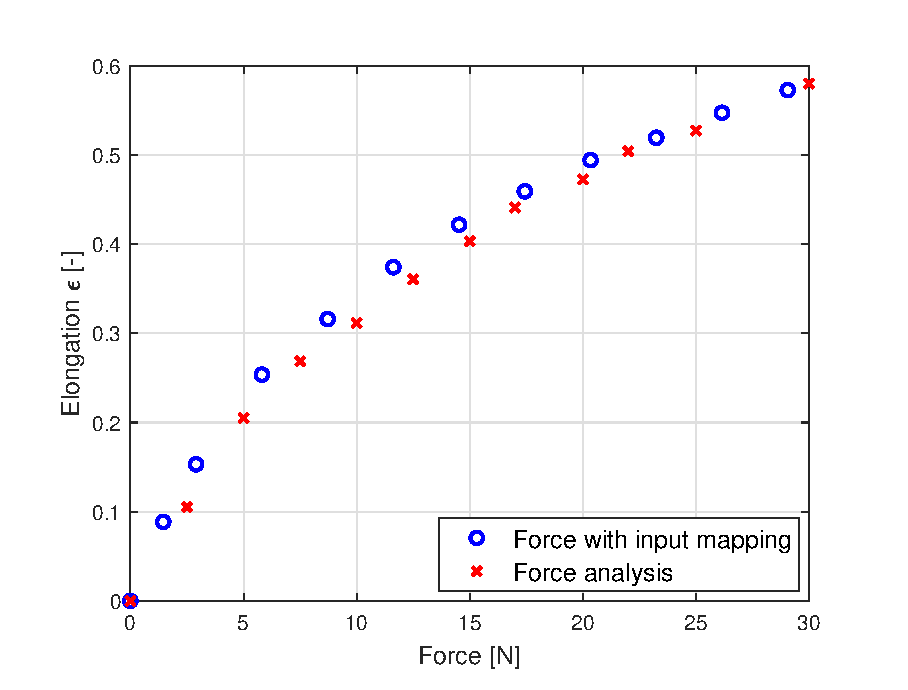
\includegraphics[width=\textwidth]{Figures/Chapter3/pressureforceelongation.eps} 
        \caption{Elongation expressed for force analysis and force with input mapping.}
        \label{fig3:forcetopressure}
    \end{minipage}
\end{figure}

The linear mapping coefficient, can be found by solving least squares problem as,

\begin{equation}
\min_{H_{2,2}} \sum_{i=1}^{N} (F_i - 2 H_{2,2} p_i)^2
\label{eq3:forcefitting}
\end{equation}

where $i$ indicates each sample point. The effective pressure area is found to be equal to 0.1462. Since $H_{2,1} = H_{2,2}$ the mapping of pressure in kPa to force in Newton is obtained. Figure (\ref{fig3:forcetopressure}) shows the results of the input mapping for the elongation. It can be seen that the pressure maps fairly accurate to the force.

Now the effective pressure area has been determined, the mapping to the moment can be calculated. It is assumed that the force acts on the top plate at a given radius form the backbone curve. The lever on which the force acts is equal to 12.56 mm, as can be seen in Figure \ref{fig3:dim}. This allows to calculate $H_{1,1}$ and $H_{2,1}$ by multiplying $H_{2,1}$ with this distance. The mapping matrix $H$ then follows as,

\begin{equation}
    H =  \begin{bmatrix} 1.8245e-3 & -1.8245e-3 \\
    0.14526 & 0.14526\end{bmatrix}  
\end{equation}


%%%%%%%%%%%%%%%%%%%%%%%%%%%%%%%%%%%%%%%%%%%%%%%%%%%%%%%%%%%%%%%%%%%%%%%%
%%%%%%%%%%%%%%%%%%%%%%%%%%%%%%%%%%%%%%%%%%%%%%%%%%%%%%%%%%%%%%%%%%%%%%%%
%%%%%%%%%%%%%%%%%%%%%%%%%%%%%%%%%%%%%%%%%%%%%%%%%%%%%%%%%%%%%%%%%%%%%%%%



\section{Stiffness properties}

The force mapping and the modal coordinates obtained through inverse kinematic optimization can be used to determine elongation and curvature stiffness. A non-linear trend in elongation and curvature as function of pressure was already observed. Therefore, it is assumed that the stiffness can be captured by the hyper-elastic stiffness model as formulated in \cite{Caasenbrood2020StiffnessModel}. This non-linear stiffness model poses that stiffness $k(q_i) \in \mathbb{R}^{\geq 0}$ and meets condition $\underbar{$k$} < k(q_i) < \Bar{k}$. The model used to describe elongation is described by,

\begin{equation}
    K_\epsilon(\alpha,q_\epsilon) =  \alpha_1 + \alpha_2 [\tanh({\alpha_3 \epsilon})^2 -1]
\end{equation}


where $\alpha_i$ and  for $i \in \{1,2,3\} $ are positive stiffness parameters to be found. It is assumed that negative pressures, e.g. creating a vacuum, result in equal elongation yet in opposite direction. Hence, self contact of the bellows is neglected. This assumption is deemed valid since this situation can not occur in our experimental set-up. The pumps used for experimental validation can not create vacuum. These stiffness parameters can be found by solving the non linear constraint optimisation described by,


\begin{equation}
\begin{aligned}
\min_{\alpha_1,\alpha_2,\alpha_3} \hspace{5pt} \sum_{i=1}^{N}(F_i -  (\alpha_1 + \alpha_2 [\tanh({\alpha_3 \epsilon_i})^2 -1])\epsilon_i)^2    \\ 
\text{s.t.} \hspace{5pt} \alpha_1 > \alpha_2 > 0 \\
\alpha_3 > 0 \\ 
\label{eq3:Keopt}
\end{aligned}
\end{equation}

which objective is to minimize the the sum of the errors between the mapped force, and force resulting from the stiffness model. As for the elongation stiffness, the curvature stiffness can be characterized by,

\begin{equation}
    K_\kappa(\beta,q_\kappa) =  \beta_1 + \beta_2 [\tanh({\beta_3 \kappa})^2 -1]
\end{equation}


where $\beta_i$ for $i \in \{1,2,3\} $ are positive stiffness parameters to be found. These parameters can be found by solving,

\begin{equation}
\begin{aligned}
\min_{\beta_1,\beta_2,\beta_3} \hspace{5pt} \sum_{i=1}^{N}(M_i -  (\beta_1 + \beta_2 [\tanh({\beta_3 {\kappa_i}})^2 -1]){\kappa_i})^2    \\ 
\text{s.t.} \hspace{5pt} \beta_1 > \beta_2 > 0 \\
\beta_3 > 0 \\ 
\label{eq3:Kkopt}
\end{aligned}
\end{equation}



where the objective is to minimize the sum of errors between the mapped moment. Solving the optimization problems described in (\ref{eq3:Keopt}) and (\ref{eq3:Kkopt}) result in the stiffness parameters as presented in Table (\ref{tab3:stiffnessparameters})

\begin{table}[H]
    \centering
        \caption{Parameters for hyper-stiffness model.}
\begin{tabular}{|c|c|c|c|} \hline
            &  $i = $ 1      &    $i = $    2   &  $i = $ 3  \\ \hline
   $\alpha_i \hspace{2pt}[N]$    &    1.3936e+3    & 1.3776e+3    & 2.7865e-1 \\ \hline
   $\beta_i \hspace{2pt}  [Nm^2] $     &  3.0322 & 3.0309    &  3.3755e-3\\ \hline
\end{tabular}
    \label{tab3:stiffnessparameters}
\end{table}

Solving the regression problem of (\ref{eq3:Keopt}) and (\ref{eq3:Kkopt}) result stiffness relation
Figure (\ref{fig3:elongvsforce}) shows the result of solving the regression problem of (\ref{eq3:Keopt})


\begin{figure}[H]
    \centering
\begin{minipage}{0.5\textwidth}
        \centering
        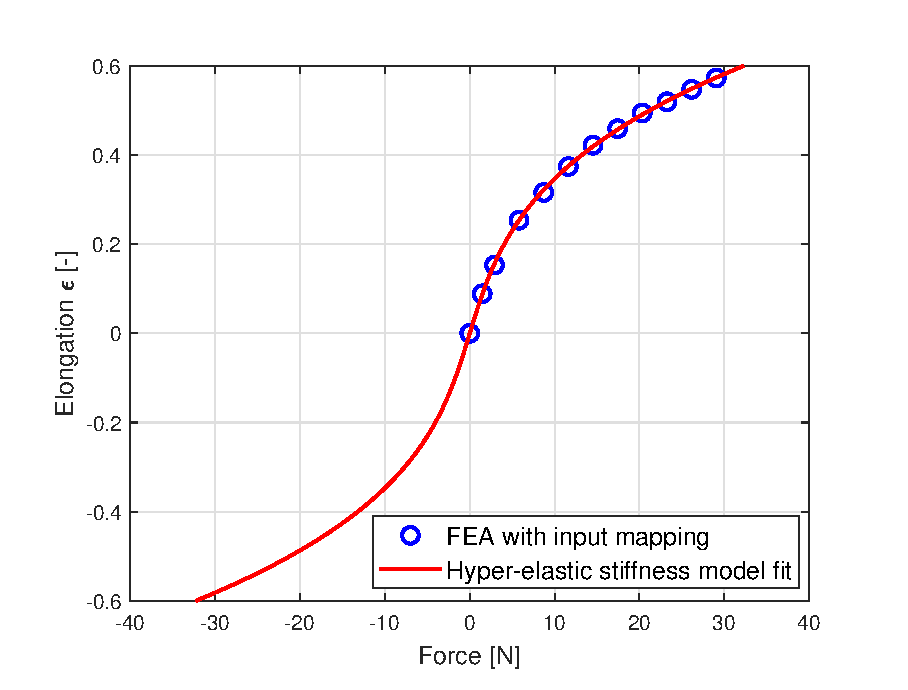
\includegraphics[width=\textwidth]{Figures/Chapter3/mappedforcevselongation.eps}
        \caption{Fitted stiffness model for elongation.}
        \label{fig3:elongvsforce}
    \end{minipage}\hfill
    \begin{minipage}{0.5\textwidth}
        \centering
        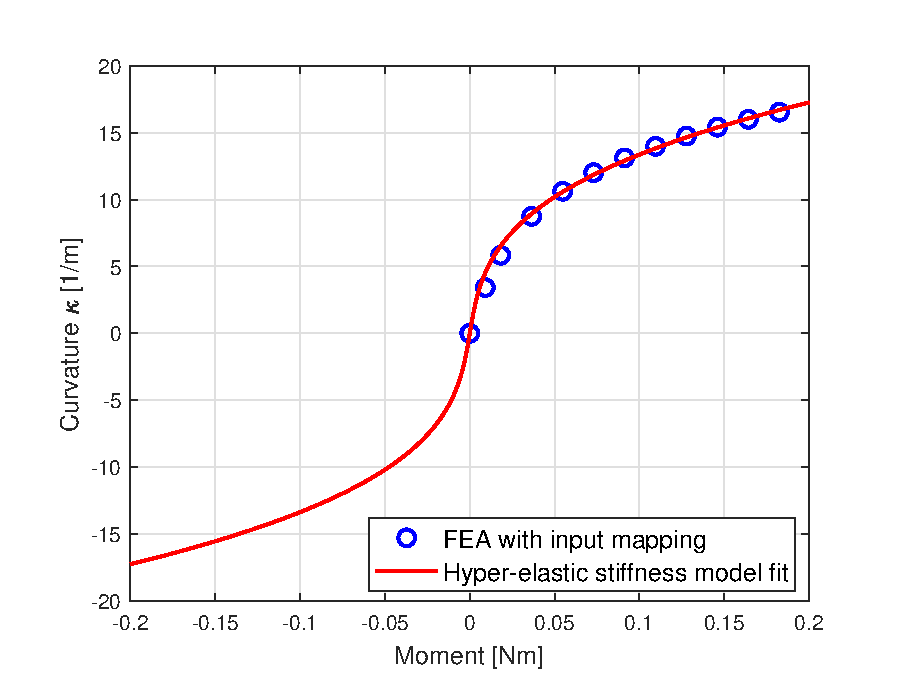
\includegraphics[width=\textwidth]{Figures/Chapter3/mappedmomentvscurvature.eps} 
        \caption{Fitted stiffness model for curvature.}
        \label{fig3:curvsmoment}
    \end{minipage}
\end{figure}






\section{Pump Dynamics}





Besides soft robot actuator properties also the actuator properties are involved. To this end the pump dynamics are determined. In the proposed control architecture, the Jacobian controller is accompanied by a pressure controller. To this end, the pump dynamics need to be determined. Initially, we determine the pump dynamics by  connecting the pump directly to the pressure sensor. This yielded poor performance once connected to the soft actuator. To suppress noise levels and capture the actual system dynamics better the set-up is slightly adapted. Furthermore we make the following assumption:


\begin{theorem}
Both air pumps have the equal pump characteristics, therefore the system dynamics of a single air pump need to be determined.
\end{theorem}


To determine the pump dynamics the pump is connected directly to the pressure sensor using a short flexible silicone hose. The pump is powered by an electric 12V DC motor, and uses membranes to create pressure. The pump characteristics are obtained by observing the systems response for various volt step inputs between 1 and 6 Volt. Although the pumps are able to operate at 12 Volt, only a maximum step input of 6V is possible for this set-up. The pressure sensor measures absolute pressures between 0 and 25 PSI, which is equivalent to a maximum of 172 kPa. Depending on weather conditions, the maximum theoretically measurable pressure is around 72 kPa. However, experiments have shown results up to 80 kPa are possible. The resulting step responses are shown in Figure (\ref{fig1:pump_dynamcis}).

\begin{figure}[H]
    \centering
    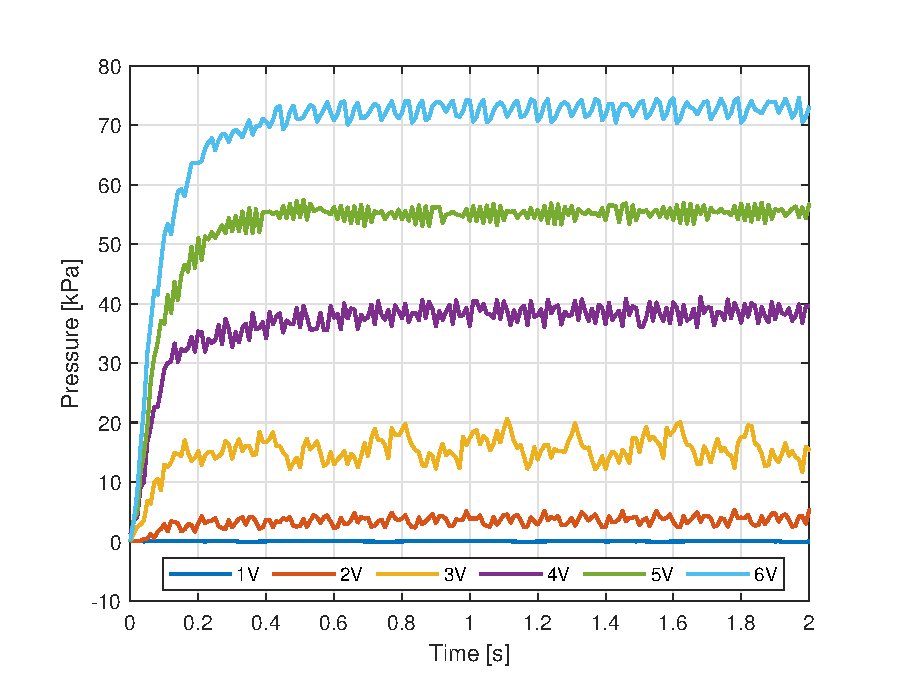
\includegraphics[width = 0.6\textwidth]{Figures/Chapter3/stepresponsdirect16V.eps}
    \caption{Step response for volt step input between 1V and 6V.}
    \label{fig1:pump_dynamcis}
\end{figure}

Multiple observations can be made based on the step response of Figure (\ref{fig1:pump_dynamcis}). A first glance reveals first order system behaviour as  pressure increase seems to be proportional to the actual pressure. However, the steady-state pressure is not proportional to the input volt for all step responses. The reason for this behaviour is thought to be friction. For 1 and 2 volt input static friction dominates, resulting in no to very small pressure increase. At 3 volt the transition between dry and kinetic friction is observed. The first order system characteristic become better visible, although the pressure response is chattering. Furthermore, we see a rise time of comparable order for step inputs of 4V and above. After around 0.5 seconds the steady-state pressure is reached. For all step inputs oscillations are observed around the steady-state pressure. This phenomena is caused by the fact that there is almost no passive leakage from the small control volume. When the pump valves open and air is pressed into the system the air waves are created. For the step input of 5 volt the valve dynamics can be clearly seen, as the dense green spikes.

An improved pump model can be obtained by altering the set-up. To this end, the actuator and an air vessel are connected to the system. Previous research showed that adding an air vessel will reduce oscillatory behaviour, at the cost of bandwidth \cite{proper}. The air vessel will increase the control volume of the entire system. When the valves open and additional air is pressed in the system, the relative pressure change is smaller. Additionally, when the actuator expands the relative volume increase will also be smaller. This will cause the system to respond slower to a step input. Furthermore, the maximum achievable pressure is lower. The addition of air vessel and actuator will increase the passive leakage of the system.

For the adapted system the step response is determined for volt steps between 2 and 12 volt. The results are shown in Figure \ref{fig3:pump_dynamics_adapted}.

\begin{figure}[H]
    \centering
    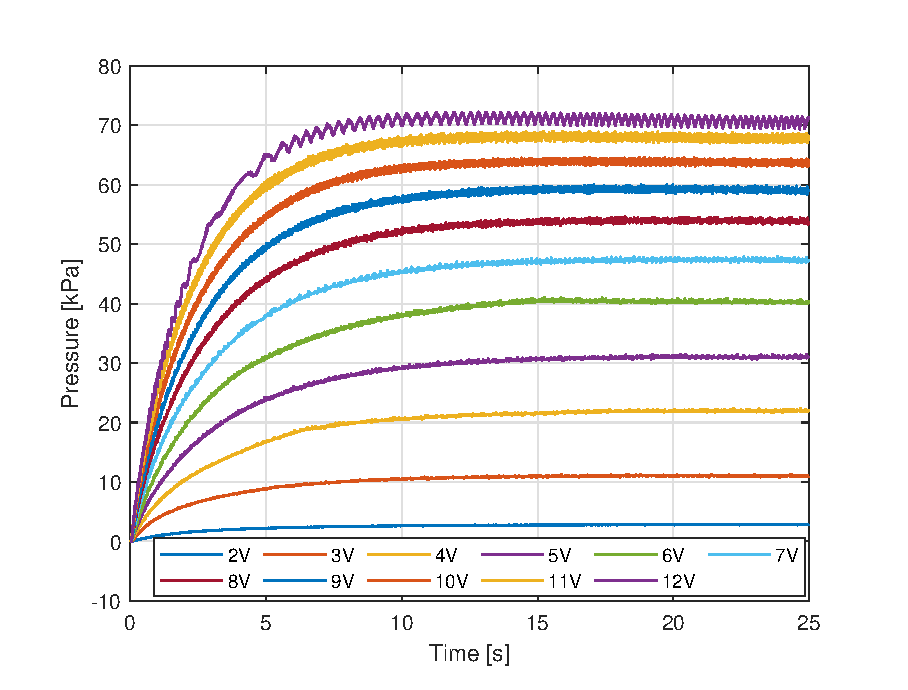
\includegraphics[width = 0.6\textwidth]{Figures/Chapter3/step212V.eps}
    \caption{Step response for volt step input between 2V and 12V for the system including air vessel and actuator.}
    \label{fig3:pump_dynamics_adapted}
\end{figure}


Based on the step responses of Figure (\ref{fig3:pump_dynamics_adapted}) we try to capture the pump dynamics in a model. The time response of a first order linear system responding to a step input is given by, 

\begin{equation}
    p(t,V) = K(1-e^{-t/\tau})V,
    \label{eq3:firstordermodel}
\end{equation}

where $p$ is the pressure at time $t$ in kPa. DC-gain $K$ [kPa/V] determines the maximum pressure, time constant $\tau_s$ [1/s] determines the growth rate of the exponential function. Furthermore, $V$ is the input volt. 

An attempt to fit the linear first order model of (\ref{eq3:firstordermodel}) did not result in an accurate description of the pump dynamics for all step inputs. Therefore an alternative description of the pump dynamics is proposed. In this description DC-gain $K$ is replaced by a nonlinear function $K(V)$. Additionally, a linear function $\tau_s(V)$ is proposed. This adaption makes the original model non-linear. Additionally, we are aware that by introducing these functions the terminology time `constant' is used incorrectly.


Based on (\ref{eq3:firstordermodel}) an indication of the gradient between constant $K$ and $V$ can be estimated. The DC-gain can be found by dividing the steady-state pressure by its corresponding volt input. The steady-state pressure for each step input is estimated by taken the mean over the last 10 seconds of data. A similar approach is done for determining time constant $\tau_s$. For a first order system it can be proven that this time constant is equal to time at which 63\% of the steady state value is reached. The corresponding relations for $K(V)$ and $\tau_s(V)$ are shown in Figure \ref{fig3:Kest} and Figure \ref{fig3:tauest}, respectively.
\newpage

\begin{figure}[H]
\begin{minipage}[b]{0.48\linewidth}
\centering
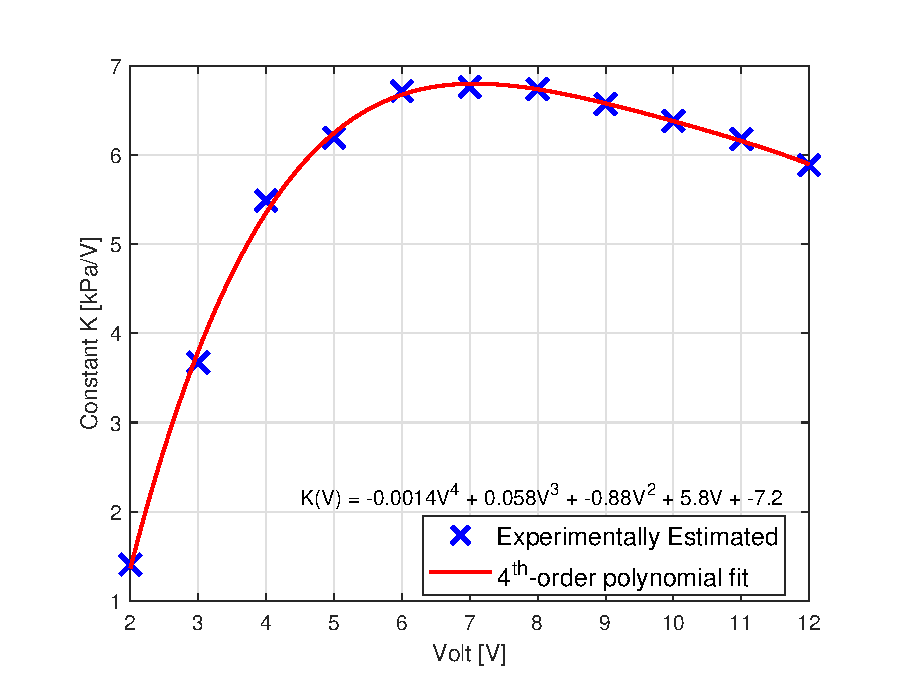
\includegraphics[width=\textwidth]{Figures/Chapter3/Kest.eps}
\caption{Experimental estimate of `constant' $K$ and fourth order fit.}
\label{fig3:Kest}
\end{minipage}
\begin{minipage}[b]{0.48\linewidth}
\centering
\includegraphics[width=\textwidth]{Figures/Chapter3/tauest.eps}
\caption{Experimental estimate of time `constant' $\tau$ and linear fit.}
\label{fig3:tauest}
\end{minipage}
\end{figure}

Figure \ref{fig3:Kest} shows a fourth-order polynomial fit through DC-gain $K$. For step inputs larger than 8 volt the DC-gain drops. This indicates that the air pump is less efficient for these volt inputs. This could be caused an increased temperature of the air pump. Another explanation for this behaviour is an increased passive leakage of the system, as steady-state pressure is higher for high volt inputs. Up till 5V the pumps do not adhere to what is expected. The DC-gains found in this region indicate inefficient pump behaviour. It is believed that this is caused by friction.

Figure \ref{fig3:tauest} shows the estimated time constants, with a linear fit. Clearly the estimated time constant for 2 and 3 volt do not follow this linear trend line. Therefore, this data point where excluded from the linear fit. A possible explanation for these outliers is the friction acting at these voltage inputs, and are therefore not reliable. Furthermore, we see the time constant decreasing for a increasing volt. This means that the pump has a faster response for higher volt input. This can make sense as the total power supplied to the air pumps is higher. 


The obtained measurement fits for $K$ and $\tau_s$ can be substituted in (\ref{eq3:firstordermodel}) resulting in an expression as,

\begin{equation}
    p(t,V) = K(V)(1-e^{-t/\tau_s(V)})V.
    \label{eq3:firstodernonlinearmodel}
    \end{equation}

The derived first order model of (\ref{eq3:firstodernonlinearmodel}) can be plotted against the experimental results of Figure (\ref{fig3:pump_dynamics_adapted}), this is shown in Figure (\ref{fig3:expvsfitpres}).

\newpage

\begin{figure}[H]
    \centering
    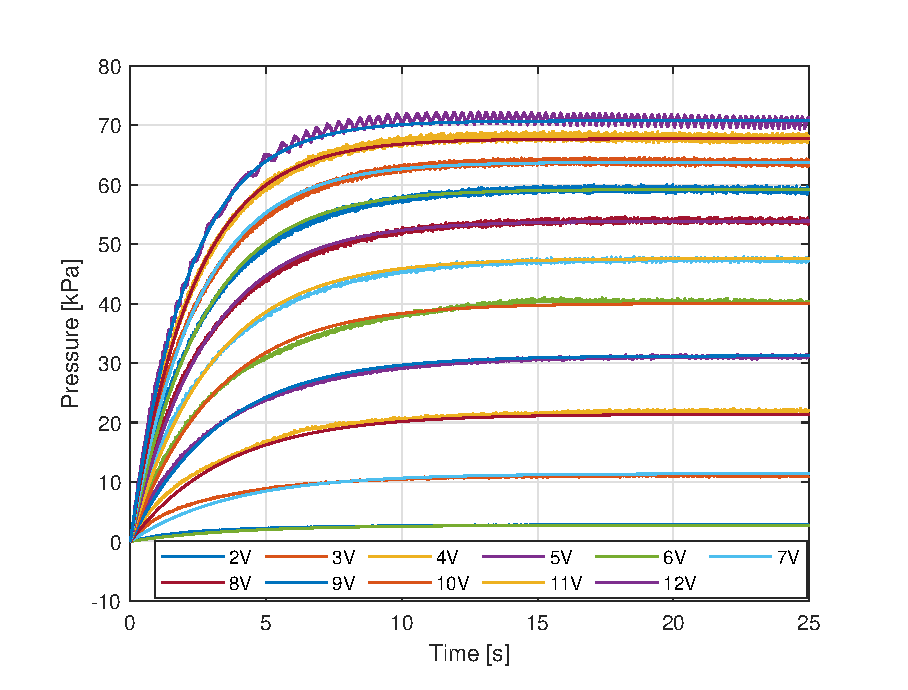
\includegraphics[width = 0.7\textwidth]{Figures/Chapter3/expfit.eps}
    \caption{Experimental results and the derived nonlinear pressure model.}
    \label{fig3:expvsfitpres}
\end{figure}

Above figure shows that the derived model captures the behaviour of the system with actuator and air vessel accurately. The steady-state pressure is close to the experimental value for all volt step inputs. As expected, the rise time for the 1 and 2 volt step inputs are not captured that well by this model.

The obtained dynamic response is arguable from a physical point of view. The dynamic model for the air pumps is fit to a first order linear system by introducing non-linearity's. Therefore the obtained model is very specific and does not allow for a change in parameters. Therefore this model can not be used in a changed set-up. Furthermore it should be noted that the fourth order fit used to describe the DC-gain is found negative for Volt input equal to 0. From a physical perspective this is not possible. At 0 volt input, the DC-gain should be equal to 0. Therefore the model is only deemed valid in the volt input range where $K$ is positive.

\hl{In this section sinusoidal response of the pump model should be added for experimental verification}



\cleardoublepage


\chapter{Controller Design}
\label{chap4}

This chapter details the controller design of the model based controller. The performance of the controller is tested with the aid of a simulation model. The model as derived in Chapter \ref{chap2} will be used with the parameters found in Chapter \ref{chap3}. In order for the model to be complete pump dynamics should be added. These pumps have a major influence on the dynamics of the system. Once these are determined the Jacobian controller can be implemented on the dynamic model. 


\section{Jacobian control}


The controller designed in this study includes jacobian information. Jacobian control is a widely used type of model-based controller for positioning classic robots. As mentioned in Chapter \ref{chapter1}, jacobian controllers only use model information on velocity and position level. Thus, system dynamics are not used in this control law.


The Jacobian controller proposed is an adapted version of the one presented in \cite{MOOSAVIAN20071226}. This work shows that a computed torque controller can be approximated by a more straightforward control law involving the Jacobian transpose. This approximation holds if high enough control gains are used. The mentioned research only uses a proportional and derivative action to reduce the error. In order to remove the steady-state error, an integrator gain is added this controller. This Jacobian transposed control law is given by,


\begin{equation}
    \nu_{set} = \begin{bmatrix}J(\sigma,t)\end{bmatrix}_1^\top \Big(K_p e + K_i \int_0^t e \hspace{2pt} ds \Big), 
    \label{eq:tau}
\end{equation}

where $\tau_{set} \in \mathbb{R}^2$ is the control input vector with control input moment and force. The Jacobian is determined with equation \ref{eq2:J}. Furthermore, $K_p$ and $K_i \in \mathbb{R}^{2\times 2}$ are diagonal gain matrices. Here $K_p$ penalizes proportional to the error, $K_i$ contributes to the sum of the error over time. The error $e \in \mathbb{R}^2$ is defined as the difference between reference position and the actual position in the (x,y)-plane. Therefore not the entire Jacobian of dimension $6 \times 2$, but only the entries mapping modal coordinate velocity to linear velocity in x-y plane. These are the fourth and sixth row of the Jacobian. As mentioned this Jacobian is space-time variant. Therefore, in the control law this Jacobian is calculated real-time based on the actual kinematic configuration of the actuator. 

The actual system does not allow to induce forces and moments directly. Therefore this control input should be mapped to pressure. Here the mapping as found with finite element analysis in Chapter \ref{chap3} is used to map pressure to force. Based on the desired control input, a reference pressure can be formulated as,

\begin{equation}
    p_{ref} = H^{-1}\tau,
\end{equation}


where $p_{ref} \in \mathbb{R}^2$ is the reference pressure for each bellow. In order for this reference pressure to be reached a second controller is necessary. This low-level controller is used to set the input voltage that is supplied to the pumps.  The volt input is regulated via pulse width modulation (pwm). Since the Raspberry PI is equipped with a 12bit ADC (analog-digital converter), it is possible calculate the pwm input as, $\textit{pwm} = \frac{2^{12} V}{V_{max}} $, where $V_{max}$ is equal to 12 volt. This control law is given by,


\begin{equation}
    pwm_{set} = K_{pp}e_p \hspace{10pt} \text{with} \hspace{10pt} e_p = p_{ref} - p,
\end{equation}



where $pwm_{set}$ is the input voltage and $K_{pp} \in \mathbb{R}^{2\times 2}$ a diagonal gain matrix. Furthermore, $e_p$ is the pressure error, which is the difference between reference pressure and actual pressure. Observe that only a proportional action is used. The integral action of the jacobian controller will already ensure no steady-state error. 




%Above state space model and presented Jacobian controller is implemented in \MATLAB. The used settings gains are $K_p = \text{diag}([400,400])$  and $K_i = \text{diag}([150,150])$. Figure  shows a simulation for a set point $q_{set} = [0 0.3]^\top$, which is equivalent to a position of [0,0.084]$m$ in the xy-plane.




%It is clear that since only a elongation is desired the pressure in both bellows should become equal. Therefore control input $V_1 = V_2$, and is saturated to the maximum 12V. Once the setpoint is nearly reached the control input slowly drops to ... V. It can be seen that the pump dynamics are the major limiting factor in the achievable performance of the set-up. The dynamic model simulations shown in Appendix \ref{app4} showed that for a free oscillation the settling time is in the order of 0.1 seconds. For this setpoint the settling time is around ... seconds. Clearly the actuator damping does not play a large role setpoint regulation. . As one can see the controller  


%Using the same tuning parameters a curvature set-point as $q_{set} = [10,0.3]$ can be simulated. 


%\begin{figure}
%    \centering
%    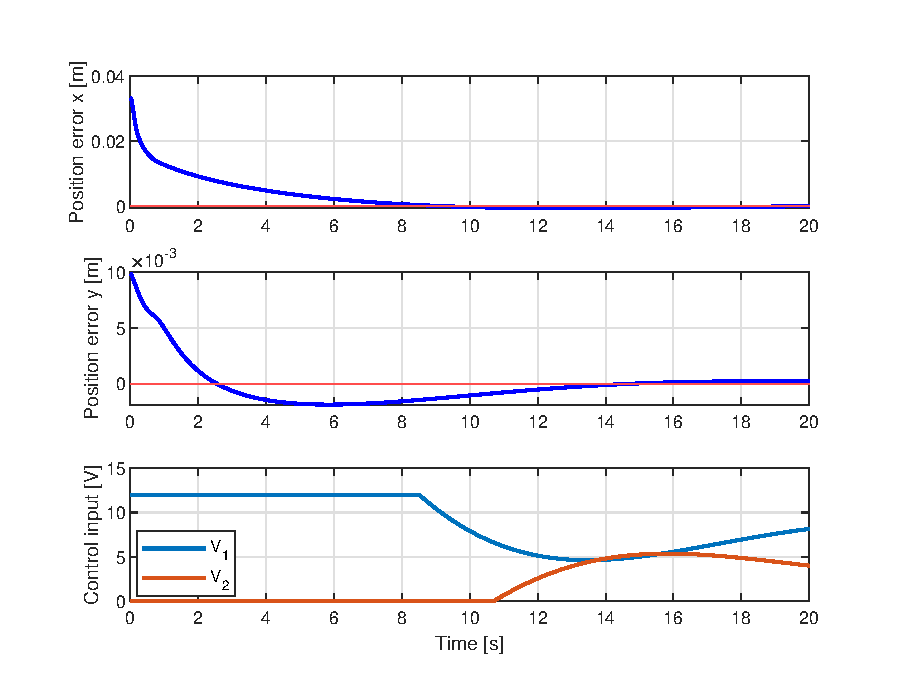
\includegraphics{Figures/Chapter4/k10e03.eps}
 %   \caption{Caption}
%    \label{fig:my_label}
%\end{figure}


























%The proposed Jacobian controller can be improved by adding additional model information. A major improving factor to the performance of the controller is adding stiffness compensation. Since the set-point is known, the necessary stiffness force and moment at that position are known. This compensation can directly be added to the control signal. The resulting controller then is,


%\begin{equation}
  %  \tau_{set} = \begin{bmatrix}J(\sigma,t)\end{bmatrix}^\top \Big(K_p e %+ K_i \int_0^t e \hspace{2pt} ds +  K_d \dot{e}\Big) + %\begin{bmatrix} K_\kappa(\kappa_{set}) & 0 \\ 0 & %K_\epsilon(\epsilon_{set}) \end{bmatrix} q_{set} , 
%    \label{eq:tauK}
%\end{equation}

%where additionally the stiffness is evaluated at modal coordinate setpoint $q_{set}$
\cleardoublepage


\chapter{Experimental Verification}
\label{chap5}



In this chapter the proposed Jacobian controller is experimentally verified. The experimental set-up will first be further detailed. This includes the data acquisition from the sensors. Then experimental results will be shown for a set-point regulation.  


\section{Experimental set-up}

The experimental set-up consisting of the planar soft robot, air pumps, airtanks, and pressure sensors are connected as followed. Each air pump is attached to an air distribution manifold via a hose. This distribution manifold has three air outlets. To these outlets a pressure sensor, air tank and actuator bellow is attached, respectively. To this end, air hoses with a inner diameter of 3mm are used. To the tip of the actuator a yellow LED used for optical tracking is mounted. This LED is glued to a connector that has been additively manufactured. The LED has an offset of 45 mm with respect the tip of the actuator. This connector part also houses the Inertial Measurement Unit (IMU). This IMU is used to measure  rotation of the actuator's tip in radians. Furthermore, a vision system is focused on the actuator. This vision system is programmed such it can recognise and track the LED marker. 

The sensors described above, e.g. the IMU, two pressure sensors and optical tracking system are connected to an Arduino micro. This Arduino is then connected to a Raspberry PI 3B+. The Arduino code is programmed such that it constantly updates all sensors. For the optical tracking system, which is the Pixy V2 the update rate is 60 Hz. The pressure sensors and IMU are read at 200 Hz. Once the Raspberry requests sensor data, the Arduino puts a string with delimiters into the Arduino serial. The Raspberry reads this string, separates the sensor data based on this delimiters, and updates the sensor data. This communication allows to reach a sampling frequency of 25 Hz. It would be more convenient to connect the sensors directly to the Raspberry. However, the Raspberry was not able to interpret this sensor data correctly. On this Raspberry the controller was programmed. To this Raspberry a ADC converter shield is mounted which can regulate the $pwm$ input to the air pumps. The programming language used for the Raspberry is \CC. For coding on the Arduino, the Arduino language is used. 

Since the position data collected by the vision system contains high-frequent noise, a first order low-pass filter was implemented on the Raspberry. This discrete low-pass filter with a cut-off frequency of 1 Hz and a sample rate of 25 Hz is given as,

\begin{equation}
    Y_k = 0.78Y_{k-1} + 0.22y_k,
\end{equation}

where $Y_k$ is new sensor value, $Y_{k-1}$ previous sensor value. And $y_k$ the new sensor data input. Notice that a zero order hold integration method is used for determining the new sensor value. 




\section{Simplified Inverse Kinematics}

The controller demands that the configuration of the actuator is known at each sampling instant. Therefore the modal coordinates need to be calculated based on the sensor data. Since the configuration of the actuator is approximated with a single shape function. The inverse kinematic problem can implicitly be solved with the constant curvature approach. The sensor output, which is the x,y position in the plane, and the orientation of the tip of the actuator $\theta$ can be used to determine modal coordinates $\epsilon$ and $\kappa$. At each sampling instant this inverse kinematics are determined. Based on the modal coordinates the Jacobian matrix can be updated, which in its turn is used in determining the new control input. The simplified kinematics are shown in Figure \ref{fig:simpkin}.

\begin{figure}[H]
    \centering
    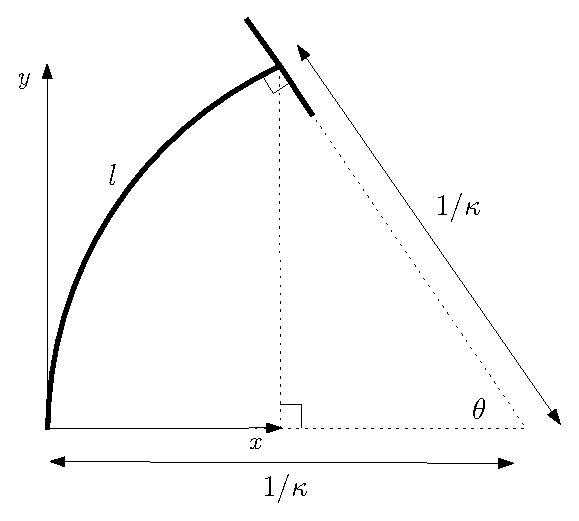
\includegraphics[width = 0.5\textwidth]{Figures/Chapter5/fbdkinematics.eps}
    \caption{Schematic drawing of the actuator to determine mapping from configuration space to task space}
    \label{fig:simpkin}
\end{figure}

From above figure the following forward kinematic relations follow as,


\begin{equation}
    y = \frac{1}{\kappa}\sin(\theta) \hspace{15pt} \text{and} \hspace{15pt}    x = \frac{1}{\kappa}[1-\cos(\theta)] \hspace{15pt} \text{with} \hspace{10pt}   \theta = l \kappa.
\end{equation}

where $l \in \mathbb{R}^{+}$ is the actuator length given by $l = (1+\epsilon)L_0$. Accordingly, the modal coordinates can then be calculated by,

\begin{equation}
    \kappa_y = \frac{\sin(\theta)}{y} \hspace{15pt} 	\land \hspace{15pt}  \kappa_x = \frac{1 -\cos(\theta)}{x} \hspace{15pt} \text{and} \hspace{10pt} \epsilon = \frac{\theta}{\kappa L_0} -1,
\end{equation}

where it should be noted that for small angles it is more accurate to use $\kappa_y$.

\section{Experimental Results}

\hl{correct experimental results are still to added.}



%\textbf{Assumptions}
%\begin{itemize}
%    \item The actuator is symmetrical, curvature equal but negative in when bellow is pressurized
%    \item Out of plane motion is negligible small
%    \item Constant curvature approach captures the kinematics well when neglecting the effect of gravity 
%\end{itemize}




\cleardoublepage

\chapter{Conclusion}
\section{Conclusion}

In this thesis, model-based feedback control applied to a single-link soft robotic manipulator is investigated. The performance of the control strategy is analyzed utilizing a simulation model and experiments. This developed simulation model incorporates the dynamics of the manipulator and air pumps. The experimental setup enabled analyzing the controller performance for real-time set-point regulation and reference tracking. This study focuses on a two-bellow soft robot actuated by air pressure. Previous work \cite{berkers} conducted on the same soft robot limited itself to linear control. In that sense, this work approached the control problem with a changed perspective. 


First, a kinematic description of the soft robot is derived based on the Cosserat beam theory. This resulted in a set of partial differential equations describing the robot configuration space. Employing a Galerkin reduction allowed to express the forward kinematics by an ordinary differential equation. The velocity kinematics are used to construct the systems space-variant Jacobian matrix. Based on Euler-Lagrange equations a non-linear dynamic model for the manipulator is derived. To capture the overall dynamics the pump dynamics as first-order systems. Combining the models resulted in an overall description of the system dynamics. 

A parameter study is conducted to obtain the stiffness properties of the soft robot. A FEM model of the soft robot is utilized to study pressure and force-induced deformation. These results are used to extract the non-linear elongation and curvature stiffness. A first-order pressure model is derived by analyzing the system's response to a sinusoidal Volt input signal. Damping properties could not be experimentally acquired.

Then a control architecture for controlling the system is designed. This architecture comprises a model-based feedback controller inspired by the soft robots space-variant Jacobian matrix. This Jacobian controller determines the pressure reference necessary to reach a given set-point in the xy-plane. The model-based controller is accompanied by a PI controller to regulate the bellow pressures. 

The control architecture is verified in simulation and experimentally. The derived dynamic model is used to tune the Jacobian controller and pressure controller in simulation. To this end, the response to a position step input is considered. For the simulation, this resulted in settling times of 16 seconds in both x and y-direction. Then the tracking of an ellipsoid reference path is studied in simulation. The noise-free simulation showed desirable tracking characteristics, with RMS errors of $0.1489 \hspace{2pt} mm$ and $0.0899 \hspace{2pt} mm$ in x and y-direction, respectively. The tracking error is caused by delays in the system. These are actuation delays caused by the pressure dynamics and control delays due to low-pass filtering of the control input. The controller is also implemented on the experimental setup. Additional filters are needed to improve sensor readings. Again, a step response is used to tune the system. The observed settling times are 12 and 8 seconds x and y-direction, respectively. The best achieved RMS errors for these step responses in x and y-direction are $0.26034 \hspace{2pt} mm$ and $0.2644 \hspace{2pt} mm$, respectively. The tracking performance is evaluated using the same reference path as in the simulation. During tracking, the achieved RMS errors are $0.7926 \hspace{2pt} mm$ and $0.4044 \hspace{2pt}  mm$ in x and y-direction, respectively. 

Conclusively, the achieved results in set-point regulation and reference tracking are satisfying. The obtained results during tracking show significant improvement with respect to \cite{berkers}. The derived dynamic model for the manipulator has shortcomings in capturing the soft robot's dynamics. However, the overall system model, which includes the pressure dynamics, compares well to the physical system. 

\section{Recommendation}

Several recommendations can be given to improve results. The following section lists improvements on the topics: modelling, setup and control design.

Firstly, improvements can be made concerning modelling. In this work, the derived dynamic model is based on a first-order Galerkin reduction, essentially reducing the model to the constant curvature approach. Although, constant curvature is a fairly accurate description of the soft robot's kinematics. The versatile Cosserat beam model can be exploited such that higher-order dynamics can also be incorporated. A higher-order reduction yields an improved representation of the theoretical infinite degree-of-freedom soft robotic system. Furthermore, it would allow studying items such as under-actuation and higher-order dynamics. Regarding this study, the mass approximation can be further improved. Although the stiffnesses seemed to be well captured, the low mass and inertia approximation led to incorrect high eigenfrequencies. Additional model improvements could be the inclusion of Coriolis effects and gravitation effects. Coriolis effects become increasingly important when the system is tuned to perform faster reference trajectories. Gravity effects are relatively simple to include in the model, and give a completer view of the actual forces acting on the system. The last model concern focuses on pressure modelling. A first-order model represents the inflation of the soft robot well. However, deflation of the actuator is neglected. Model-wise this can also be included by a first-order linear deflation model. 

In terms of setup, several improvements can be made. First of all the system can not be actively deflated. Therefore deflation rates are an important limitation when it comes to high-speed reference changes. To overcome this limitation a controllable valve could be added to the setup to deflate the bellows quickly. Also, the choice can be made to introduce vacuum pumps to deflate the soft robot's bellows. When it comes to air pumps a major improvement can also be the introduction of pressurized vessels. Contrary to diaphragm pumps, pressurized vessels allow for a constant inflow of air. Therefore it would remove the valve dynamics entirely. Furthermore, it would allow for quicker inflation which can improve performance. Additionally, air pumps saturation limits do not need to be taken into account anymore. Other improvements can be made for data acquisition. A major limitation is the sampling frequency due to serial communication between the Raspberry PI and Arduino. Desirably, all control actions and sensor readings would be done by the Raspberry. This would increase the sampling frequency and allows for real-time evaluation of the results. The current vision system has a 60 Hz update rate, which is a considerable limitation when demanding higher performance. In this study, a low-pass filter is used to give a better position estimate. However, this does add additional delays in the system. Therefore a higher update rate and higher resolution can be beneficial. A final improvement on the setup is the LED marker, in this study a yellow LED is used. However, the hue value is close to the soft robot's hue. Therefore, vision system tuning is cumbersome. It would be better to replace this LED with another coloured LED. 


Lastly, there is a lot of performance to be gained with improving the control architecture. In this study, only a feedback controller is considered. In soft robotics, feedback control conflicts with the intrinsic properties of soft robotics. Feedback control namely introduces stiffness, whilst the soft robot is designed to be flexible. To reduce this effect and enhance performance, feedforward can be introduced. In the current control architecture, the pressure reference increases slowly as a result of the integrator action. Since stiffness models are available, the addition of stiffness compensation in the Jacobian controller will ensure a faster increase of pressure set point. Together with a feedforward model on the pumps, this will allow for faster reference tracking. Another improvement would be the inclusion of gravity compensation. Of course, control methods that involve a more model-based approach can be implemented. Promising methods, especially for under-actuated systems, include computed-torque control, (partial) feedback linearization and passivity-based control.  

\cleardoublepage

%\chapter{Questions}
%\section{week 2}


The code has been altered. Unfortunately it doesn't work for NMODE = 1 again. What has exactly changed to the code, so I can solve this problem quicker? \\



Do you know what program can be used for making free body diagrams such as fig 3.1 (Has thesis) pag. 20 and fig 3.6 pag.24\\


I was thinking of using another way of validating the model. I was trying to use a laser distance sensor and measure elongation. However, this means that we can measure 2 dof, rotation and elongation, separately. As there is no way of measuring both dof simultaneously using the laser distance sensor. This did not seem possible now, therefore I want to conduct the experiment with



read dynamic control of the BHA falkenhan



abaques, pressure simmulation, table, fit Kx = tau

\section{week 3}

connector parts Has, used your 3D printer as well? Rethink about connector design tomorrow.

CAD files from the planar robots?

sluit jij de pressure sensors aan / voeg jij ze toe aan de set-up?



\section{week 4}


rotations gaan nog mis, als er een uitwijking in negatieve x gewenst is. Oplossing?






\newpage
\bibliography{bibliography}
\bibliographystyle{unsrt}
\cleardoublepage

\begin{appendices}

%\appendix
\chapter{Dynamic Modelling}
\section{Inverse kinematics}
\label{app:chap2}

%This subsection is not definite. 2 inverse kinematic scripts have been created. One in which only end-effector position $[x,y]$ is given. One where also the orientation is added $[x,y,\theta]$ . For only a single shape-function approximation (constant curvature approach), will find the shortest path. However, when increasing the amount of shape functions, both models will not come with the most shortest path. Therefore, the inverse kinematics as described here has not been used extensively.


Inverse kinematics allows to map the desired end-effector position to the corresponding modal coordinates. To determine this inverse mapping the Jacobian search method is exploited \cite{JacobianInverse}. Essentially, a desired position and orientation of the robot's end-effector is given. 


The derived forward kinematics can be regarded as,

\begin{equation}
    x = f(q),
\end{equation}

where, $x \in \mathbb{R}^n$ is the position and orientation vector of the end-effector. For the planar robot $n = 3$, as two translations and one coupled rotation can be achieved. Here, $f$ represents the forward kinematics mapping the modal coordinate $q \in \mathbb{R}^m$ to the end-effector position. Where $m$ depends on amount of shape functions used to describe a given strain. The inverse kinematic problem aims to find a mapping $q\mapsto x$. This mapping is obtained by exploiting the inverse jacobian method according to an iterative updating scheme as,

\begin{equation}
    q_{k+1} = q_k + \chi [J(\sigma)]_1^\dagger Q e_k \hspace{20pt} \text{with} \hspace{10pt}  e_k = x_d - x_k,
    \label{eq2:qupdate}
\end{equation}

where $q_k$ is modal coordinate vector at iteration $k$, $\chi > \mathbb{R}^+$ a learning gain to enhance fast convergence $Q \in \mathbb{R}^{n\times n}$ is a diagonal matrix used to prioritize desired end-effector coordinates. In our case, the position is prioritized over the orientation. Lastly, $J^\dagger$ is an adapted form of the damped Moore–Penrose pseudo inverse defined as,

\begin{equation}
    J^\dagger = WJ^\top(JWJ^\top + \mu^2 I)^{-1}
    \label{eq2:pseudoinverse},
\end{equation}

where $W \in \mathbb{R}^{m\times m}$ is a diagonal weighing matrix that can be used to stress lower order shape functions. Put in other words, the algorithm aims to achieve the same error norm while prioritizing modal coordinates belonging to lower order shape functions. This can be used to decide on the amount of shape functions used in approximation. The factor $\mu^2 I \in \mathbb{R}^{6 \times 6}$ is introduced to avoid singularities of the jacobian matrix $J \in \mathbb{R}^{6 \times m}$. 

An algorithm capable of finding a inverse kinematic solution is created based on Equation (\ref{eq2:qupdate}). The algorithm is initiated with a desired end-effector position $x_{set}$ and guess for modal coordinates $q_0$. Furthermore, the amount of shape functions used to approximate the end-effector position is user defined. This results in,


\begin{algorithm}[H]
\caption{Numerical Inverse Kinematics}
\begin{algorithmic}[1]
\State $q$ $\leftarrow$ $q_0$ \Comment{Initial condition}
\While{$|| x_{set} - x_k || > \delta$}{}      \Comment{While error is larger than some $\delta$}
    \State $x_k$ $\leftarrow$ $f(q_k)$  \Comment{Position at current generalized coordinate}
     \State $e_k$ $\leftarrow$ $x_k - x_{set}$ \Comment{Current error}
        \For{$0:\Delta \sigma:L$}
            \State $J_{\sigma}$ $\leftarrow$  $J_{\sigma}$ + $Ad_{g(\Delta \sigma)} B_a \Phi(\Delta \sigma)$ \Comment{Numerical integration over length L}
        \EndFor
    \State \textbf{end}
    \State $J$ $\leftarrow$ $Ad_{g^{-1},\sigma=L}$ $J_{\sigma}$ \Comment{Compute Jacobian}
    \State $J^{\dagger}$ $\leftarrow$  $w$ $J^{\top}$ $(J^\top w J - \mu^2 \mathbb{I}_3)^{-1}$ \Comment{Calculate pseudo inverse}
    \State $q_{k+1}$  $\leftarrow$ $q_{k}$ + $\chi$ $J^{\dagger} Q e_k$ \Comment{Update generalized coordinates}
\EndWhile 
\State \textbf{end}
    \label{alg2:numericalinverse}
\end{algorithmic}
\end{algorithm}


\section{Velocity kinematics}


Using the equality of mixed partial derivatives, at each instant of space and time $\frac{\partial}{\partial t}g' = \frac{\partial}{\partial \sigma}\dot{g}$ holds \cite{Caasenbrood2020}. Substituting (\ref{eq2:dgdsigma}) and (\ref{eq2:dgdt}) into this relation and simplifying results in,

\begin{equation}
    \hat{\eta}' = -(\hat{\xi}\hat{\eta} - \hat{\eta}\hat{\xi}) + \Dot{\xi},
        \label{eq2:pde2}
\end{equation}

here the Lie bracket $\xi$ and $\eta$ can be recognized between the parenthesis. The Lie bracket $[\hat{\xi},\hat{\eta}]$ also belongs to the group of Lie algebra $\mathfrak{se}(3)$. Therefore, it can be expressed by the adjoint action between $\xi$ onto $\eta$. This adjoint action maps the PDE of (\ref{eq2:pde2}) from $\mathbb{R}^{6\times 6}$ to $\mathbb{R}^6$. This allows to write the velocity kinematics in vector notation as,

\begin{equation}
    \eta'= -\text{ad}_\xi \eta + \Dot{\xi} \hspace{10pt} \text{with} \hspace{10pt} \text{ad}_{\xi} = \begin{bmatrix} K_\times & 0_{3\times 3} \\ E_\times & K_\times \end{bmatrix}.
    \label{eq2:etapde}
\end{equation}


Exploiting the relation $\frac{d}{d \sigma} \text{Ad}_g = \text{Ad}_g \text{ad}_{g^{-1}g'}$ \cite{Boyer2019}, \cite{traversaro2016multibody} , with $g^{-1}g' = \xi$ which follows from (\ref{eq2:dgdsigma}), it follows that $-\text{ad}_\xi = (\text{Ad}_g^{-1})'\text{Ad}_g$. Substitution of this expression into (\ref{eq2:etapde}) allows to formulate the spatial derivative of the velocity twist as,

\begin{equation}
    \eta'= (\text{Ad}_g^{-1})'\text{Ad}_g \eta + \Dot{\xi} \hspace{10pt} \text{with} \hspace{10pt} \text{Ad}_g = \begin{bmatrix} R & 0_{3\times 3} \\ p_\times R & R \end{bmatrix}
    \label{eq2app:etadif}
\end{equation}

where $\text{Ad}_g \in \mathbb{R}^{6 \times 6}$ and $\text{Ad}_{g^{-1}}  \in \mathbb{R}^{6 \times 6}$ are the adjoint and inverse adjoint mapping of $g$, respectively \cite{Sola2018}. An analytic solution can be found by integrating (\ref{eq2app:etadif}) over spatial domain $[0,\sigma]$. However, solving PDE's is generally more computationally expensive and makes controller design hard.
To overcome this, the theoretical infinite dimensional system is projected onto a finite dimensional subspace. In order to do so, we assume the following.

\cleardoublepage

%\appendix
\chapter{Stiffness Determination}
\label{app:chap3}


\section{Mesh refinement analysis}

Proper meshing is crucial in order to obtain accurate simulation data. Coarse meshes will generally result in poor results that badly represent the deformation of the system. Fine meshes will consume a lot of RAM and therefore take up a lot of computation time. Therefore, a valid mesh size needs to be obtained, which balances the accuracy of output data and computation time. To this end, multiple simulations are carried out in $\verb+Abaqus/CAE+$ to justify the mesh size.

In the simulation, both bellows are pressurized to $80$ kPa. Multiple simulations are carried out for an increased amount of nodes. These nodes are a measure for the mesh size. The elongation of the manipulator is determined for each simulation. Figure \ref{fig3:meshrefinement} shows the determined elongation as a function of the number of nodes.

\begin{figure}[H]
    \centering
    \includegraphics[width = 0.6\textwidth]{Figures/Chapter2/MeshRefinement.eps}
    \caption{Mesh refinement analysis for a bellow pressure of $80$ kPa.}
    \label{fig3:meshrefinement}
\end{figure}


Figure \ref{fig3:meshrefinement} shows that from 60 thousand nodes onwards the elongation data may be deemed reliable. A lower amount of nodes results in poor data output. Furthermore, it can be seen that increasing the number of nodes does not improve the simulation output any further. At 60 thousand nodes, the elongation has already converged.




\cleardoublepage

%\appendix
\chapter{Controller Design}
\label{app4}


\section{Dynamic Model}

Since damping parameters can not be obtained experimentally, it was opted for to intuitively tune these gains based on observations in the lab. This assumption is deemed valid as the pump dynamics are dominant for set-point regulation tasks. In this section we compare the dynamic system for a free oscillation for two different damping settings. A critically damped system, which resembles observations made in the lab best. And a under damped system, to illustrate other dynamical characteristics of the system. For both simulations the initial conditions where a curvature of $8$ $\frac{1}{m}$ and elongation of $0.5$ $[-]$.


Figure \ref{figapp4:highd} shows a free oscillation of the dynamic model with damping constants $D_\kappa = 4\mathrm{e}{-5} Nms$ and $D_\epsilon = 0.3 Ns $. This results in a critically damped system. There is no oscillatory behaviour around the steady-state. These settings represent the actual system best. It can be seen that the system settles the order of 0.1 seconds.

Figure \ref{figapp4:lowd} shows a free oscillation of the dynamic model with damping constants $D_\kappa = 2\mathrm{e}{-6} Nms$ and $D_\epsilon = 9\mathrm{e}{-3} Ns $. This results in a under damped system. This simulation is added to show the effects of the non-linear stiffness, which is indicated by the inconsistent width of the oscillations.

\begin{figure}[H]
\begin{minipage}{0.48\textwidth}
    \centering
    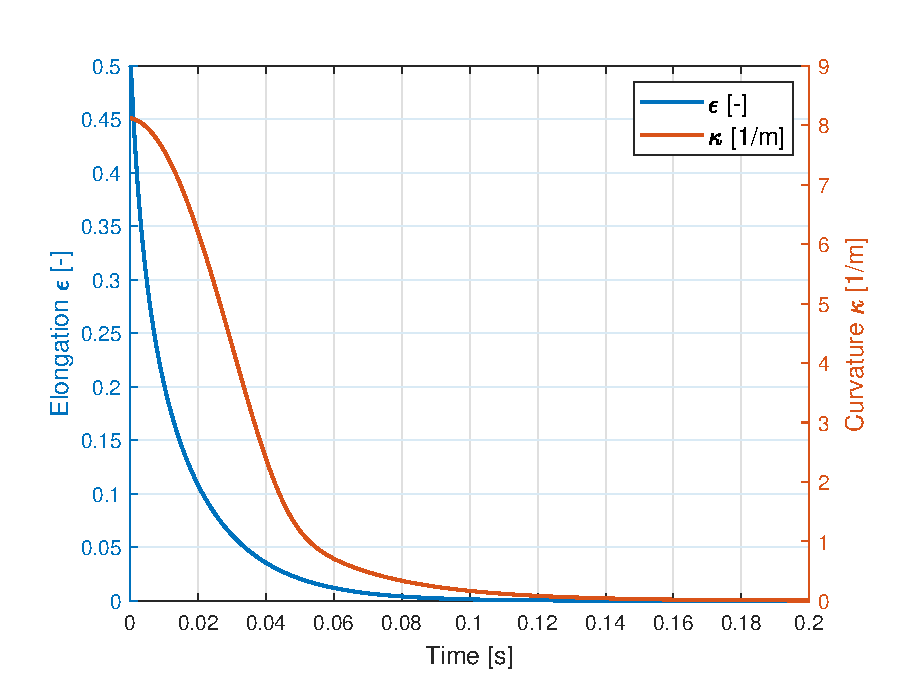
\includegraphics[width = \textwidth]{Figures/Chapter4/freeoschighd.eps}
    \caption{Free oscillation of the dynamic model with $q_0 = [8,0.5]$ for relatively high damping}
    \label{figapp4:highd}
    \end{minipage}
\begin{minipage}{0.48\textwidth}
    \centering
    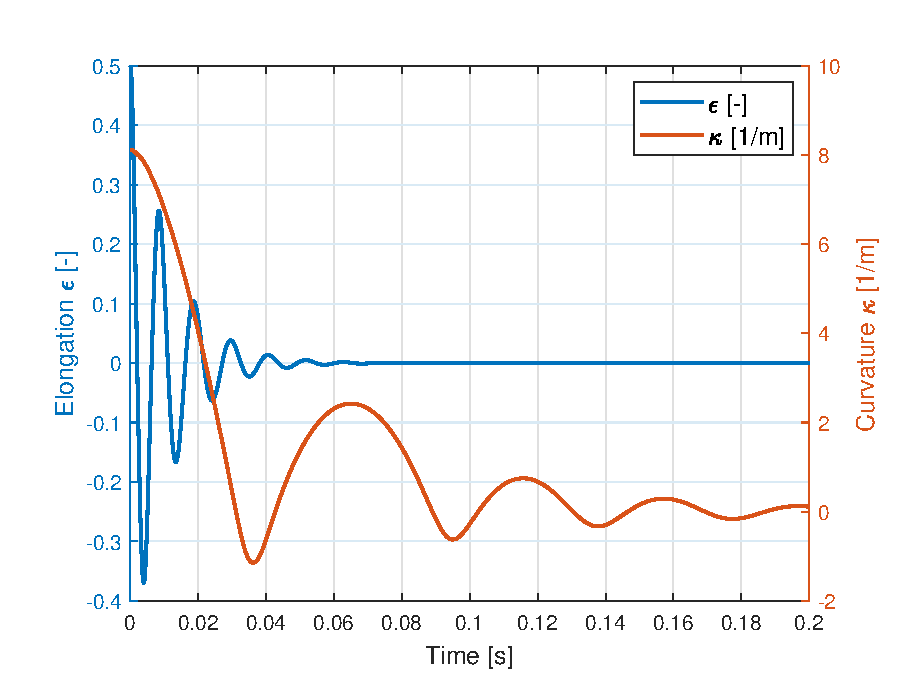
\includegraphics[width = \textwidth]{Figures/Chapter4/freeosclowd.eps}
    \caption{Free oscillation of the dynamic model with $q_0 = [8,0.5]$ for relatively low damping}
    \label{figapp4:lowd}
    \end{minipage}
\end{figure}
\cleardoublepage
\end{appendices}



\end{document}
